\documentclass[landscape,footrule]{foils}
\usepackage[lecture-serie]{foiltex-extra}
\usepackage{crysymb}
\usepackage{graphics}
\usepackage[pdftex]{graphicx} 
\usepackage{soul}
\usepackage{xcolor}
\usepackage[normalem]{ulem}




\newcommand{\lecture}{Expectation-maximisation algorithm}
\newcommand{\lserie}{LTAT.02.004 Machine Learning II}
\newcommand{\ldate}{May 8, 2019}
\newcommand{\lauthor}{Sven Laur}
\newcommand{\linst}{University of Tartu}
\graphicspath{{./illustrations/}}
\MyLogo{\lserie,\  EM algorithm, \ldate}


\newcommand{\leqm}{\ \leq_m}

%:
\newcommand\redsout{\bgroup\markoverwith{\textcolor{red}{\rule[0.3ex]{2pt}{4.0pt}}}\ULon}

\newcommand{\bigvskip}{\vskip 2em}
\newcommand{\lastline}{\vspace*{-2ex}}
\newcommand{\spreadappart}{\vspace*{\fill}}


\newcommand{\pd}[1]{\mathrm{p}[#1]}
\DeclareMathOperator*{\argmax}{argmax}
\DeclareMathOperator*{\argmin}{argmin}


\begin{document}
\titlefoil

\foilhead[-1cm]{Quick recap of hard clustering}

%\enlargethispage{1cm}

\textbf{Model.}
A hard-clustering algorithm is based on a probabilistic model
\begin{align*}
\pd{\vec{x}_1,\ldots,\vec{x}_n|\vec{z},\vec{\Theta}}
\end{align*}
where $\vec{z}$ denotes \emph{unknown} labels  and $\vec{\Theta}$ captures all model parameters. 
%\vspace*{1cm}

\textbf{Optimisation task.} The aim of hard-clustering algorithm is to minimise 
\begin{align*}
F(\vec{z},\vec{\Theta})=-\log \pd{\vec{x}_1,\ldots,\vec{x}_n|\vec{z},\vec{\Theta}}\enspace.
\end{align*}
If all data points are independent form each other then we can  simplify
\begin{align*}
F(\vec{z},\vec{\Theta}) =- \sum_{i=1}^n \log\pd{\vec{x}_i|z_i,\vec{\Theta}_{z_i}}
\end{align*}
where $\vec{\Theta}_{z_i}$ denotes parameters for the $z_i$th data source.\vspace*{-0.5cm}


\foilhead[-1cm]{Two-step minimisation algorithm}



\textbf{M1 step.} Find a new labelling $\vec{z}$ that minimises $F(\vec{z},\vec{\Theta})$ for fixed $\vec{\Theta}$. Due the form of $F(\vec{z},\vec{\Theta})$ the label can be sought for each data point separately:
\begin{align*}
 z_i=\argmax_{z\in\set{1,\ldots,k}} \pd{\vec{x}_i|z_i=z,\vec{\Theta}_{z}}\enspace.
\end{align*}


\textbf{M2 step.} Find parameters $\vec{\Theta}$ that minimise $F(\vec{z},\vec{\Theta})$ for fixed $\vec{z}$. Again, parameters can separately be sought for each data source:
\begin{align*}
 \vec{\Theta}_j^*=\argmax_{\vec{\Theta}_j} \sum_{i\in\III_j}\log \pd{\vec{x}_i|z_i=j,\vec{\Theta}_{j}}\enspace
\end{align*}
where $\III_j=\set{i: z_i=j}$ denotes elements coming form the $j$th data source.


\foilhead[-1cm]{Illustrative example}
\begin{center}
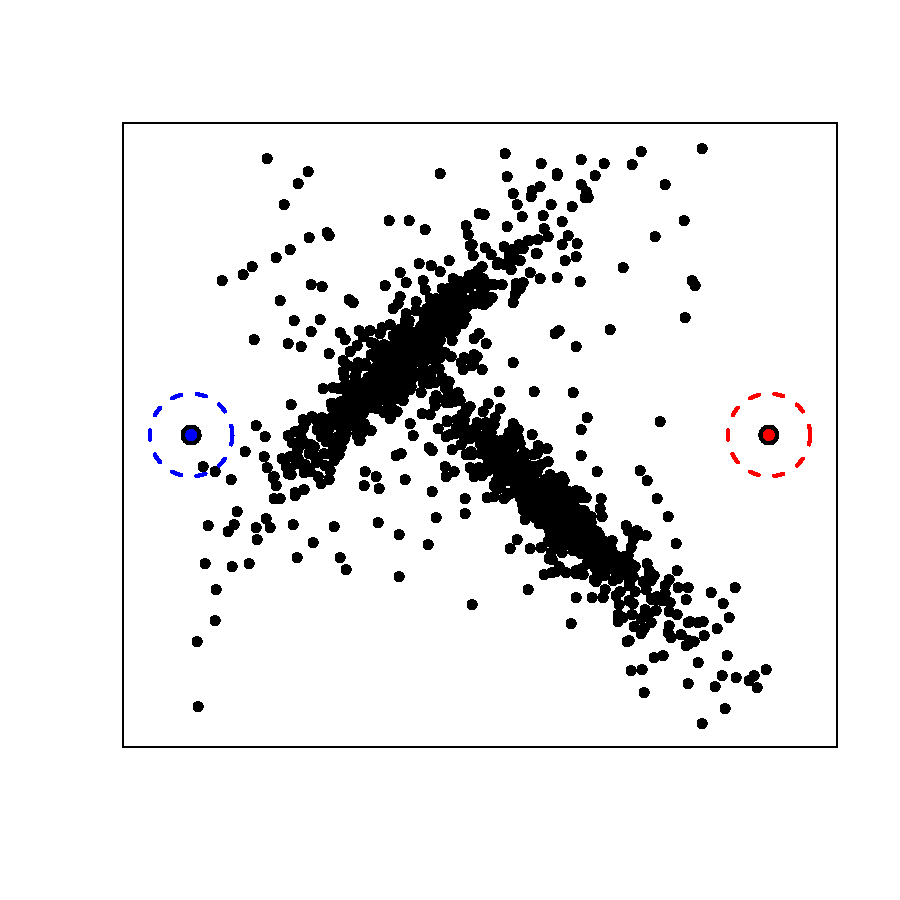
\includegraphics[width=7.5cm]{hard-gmm-1}\hspace*{-1cm}
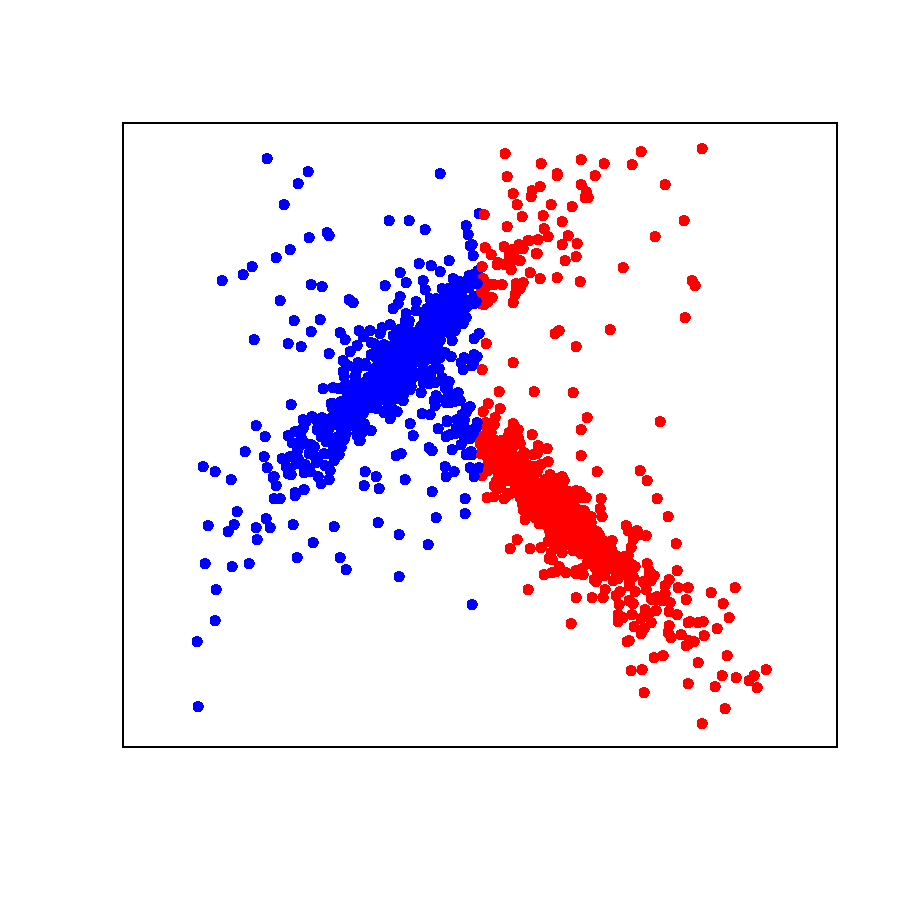
\includegraphics[width=7.5cm]{hard-gmm-2}\hspace*{-1cm}
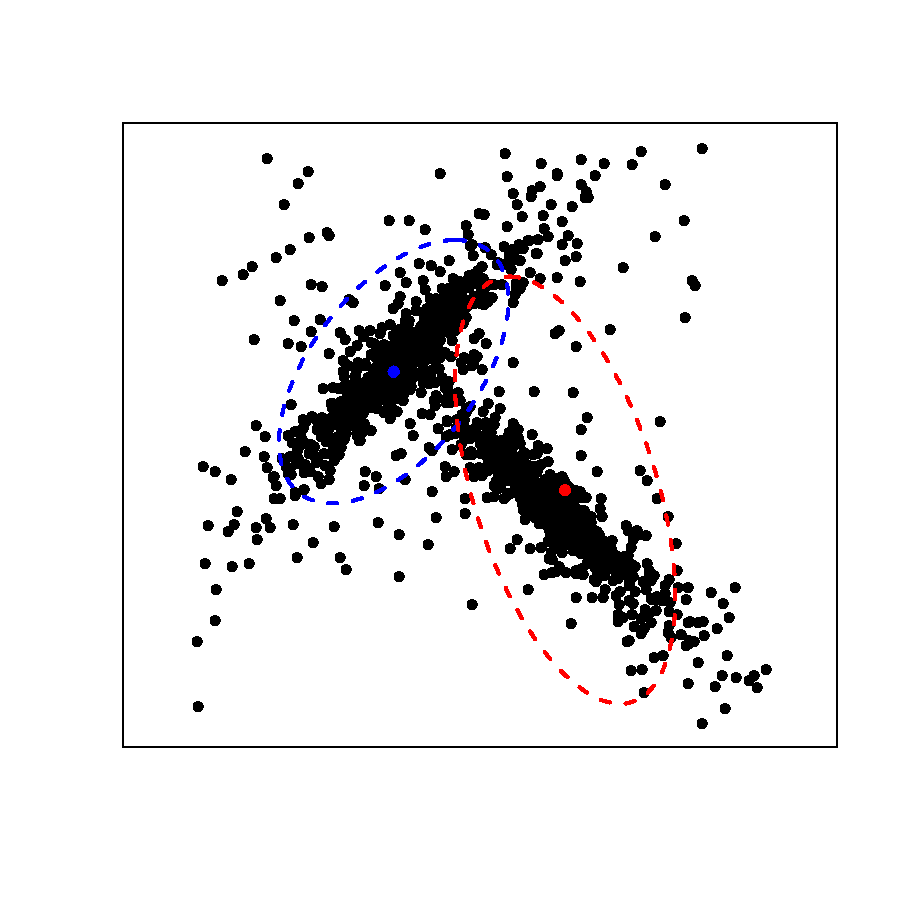
\includegraphics[width=7.5cm]{hard-gmm-3}
\vspace{-2cm}

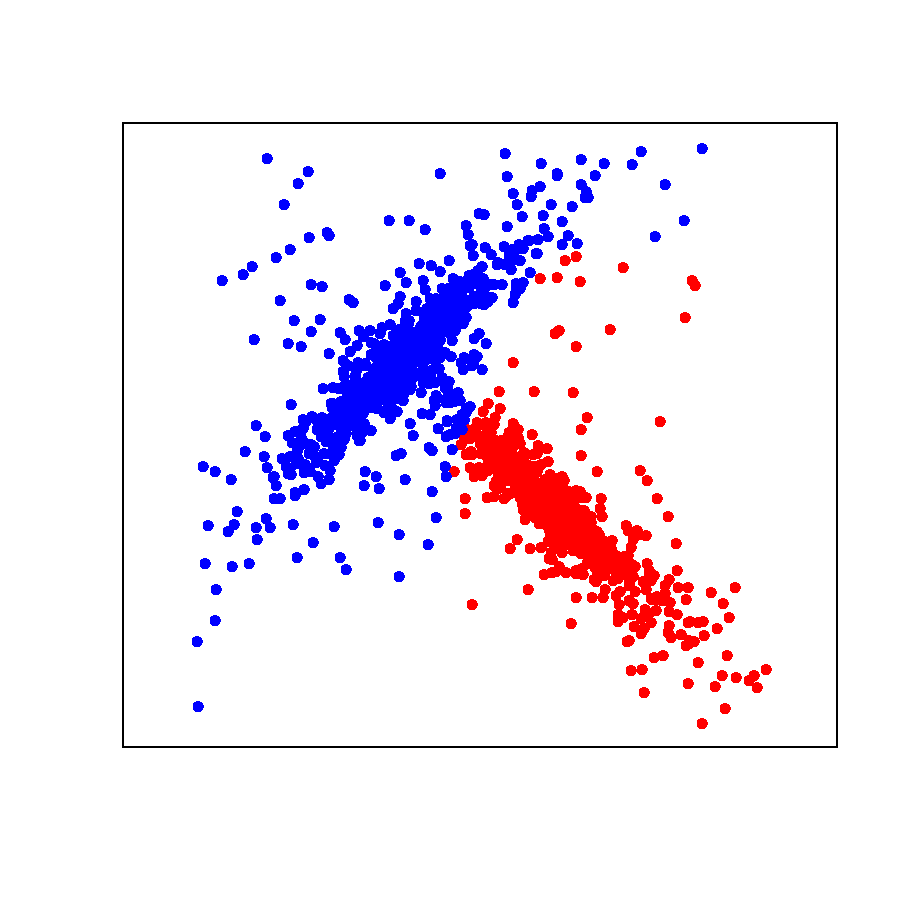
\includegraphics[width=7.5cm]{hard-gmm-4}\hspace*{-1cm}
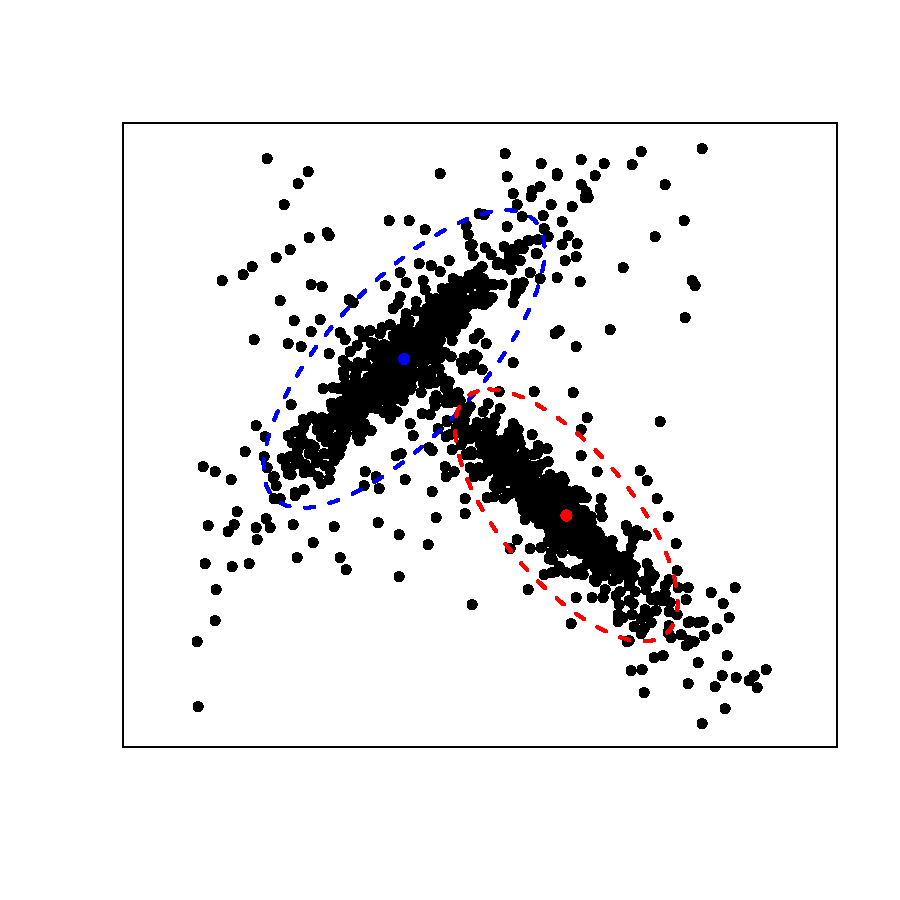
\includegraphics[width=7.5cm]{hard-gmm-5}\hspace*{-1cm}
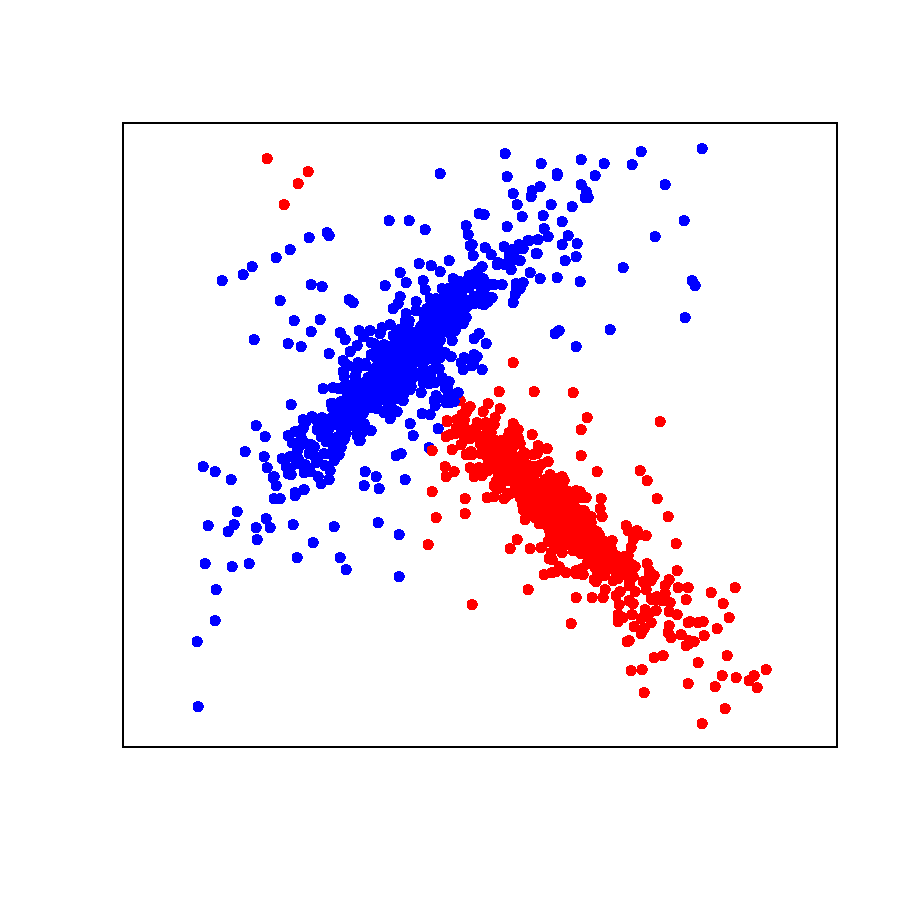
\includegraphics[width=7.5cm]{hard-gmm-6}
\vspace*{-1cm}
\end{center}


\foilhead[-1cm]{Hard clustering is brittle against outliers}
\begin{center}
\hspace*{-1cm}
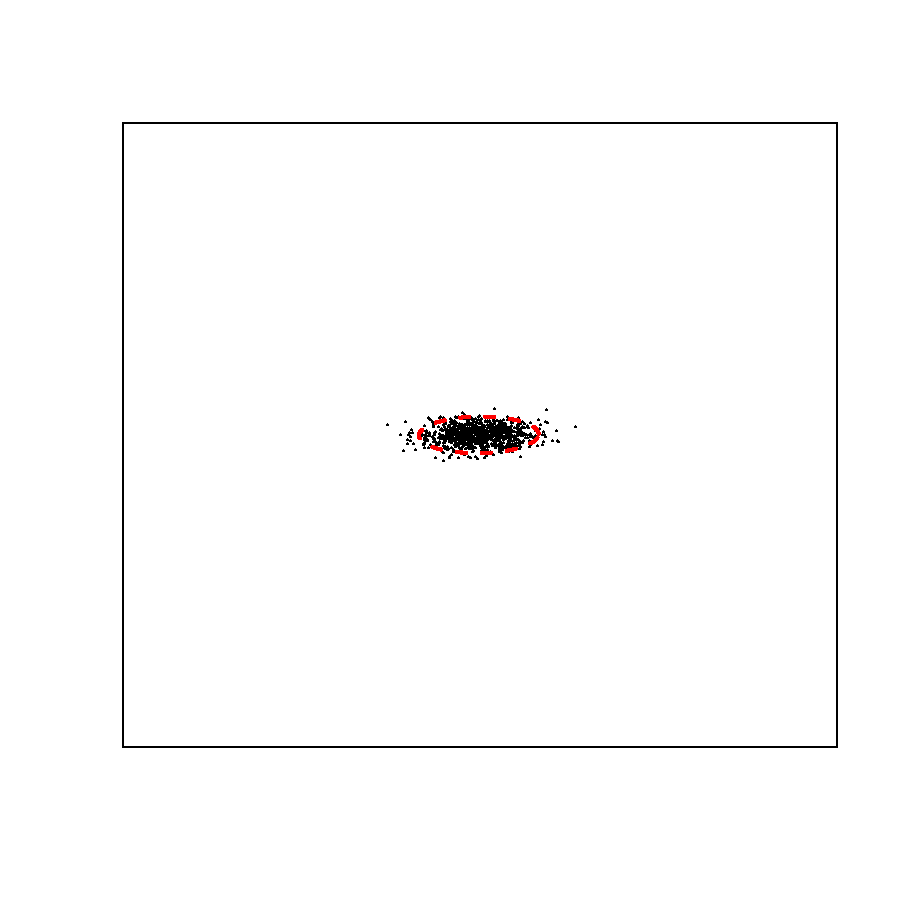
\includegraphics[width=12cm]{corrupted-gmm-1}\hspace*{-2cm}
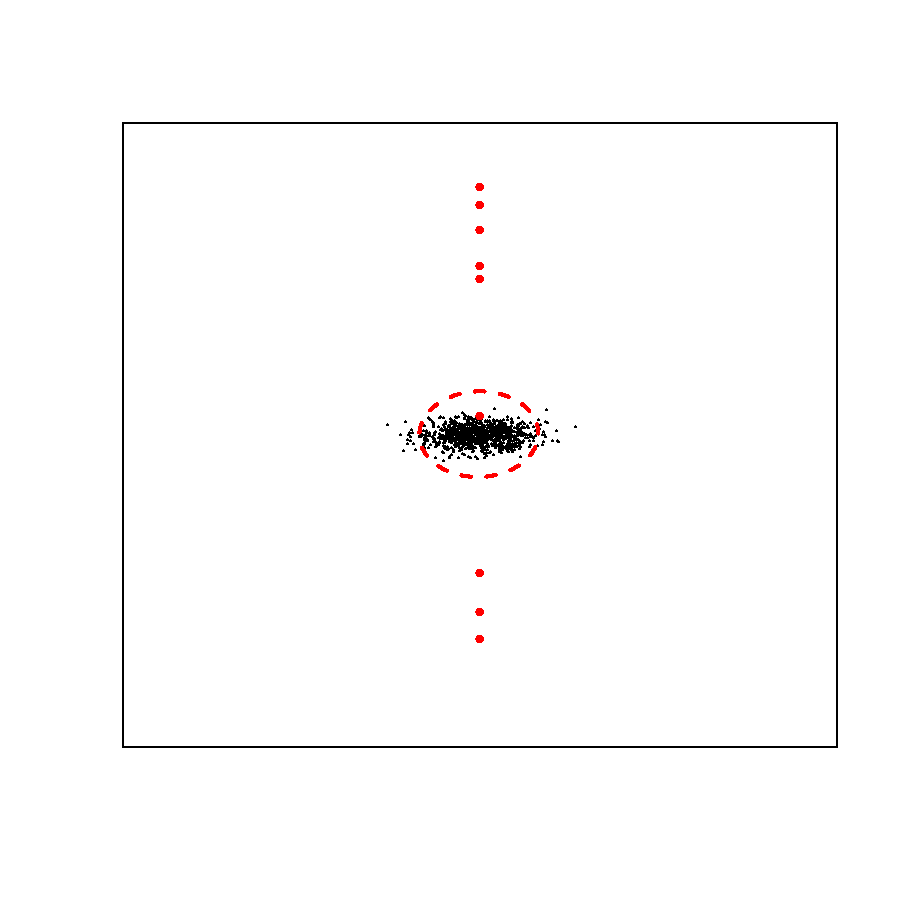
\includegraphics[width=12cm]{corrupted-gmm-2}
\end{center}
\vspace*{-2cm}
A few data points not belonging to the cluster can completely offset the shape estimation procedure. We need to reduce the impact of  outliers.\vspace*{-1cm}

\foilhead[-1cm]{Quick fix}

Assuming that current parameter estimates are not far off, we can make parameter fitting more robust by throwing out improbable points.
\begin{triangles}
\item Compute likelihood $\pd{\vec{x}_i|\vec{\Theta}_j}$  for each data point $\vec{x}_i$ in the cluster
\item Throw out $5$-$10\%$ cluster points with lowest likelihood scores
\item Model parameters based on the reduced dataset 
\end{triangles}

\foilhead[-1cm]{Illustrative example}

\begin{center}
\hspace*{-1cm}
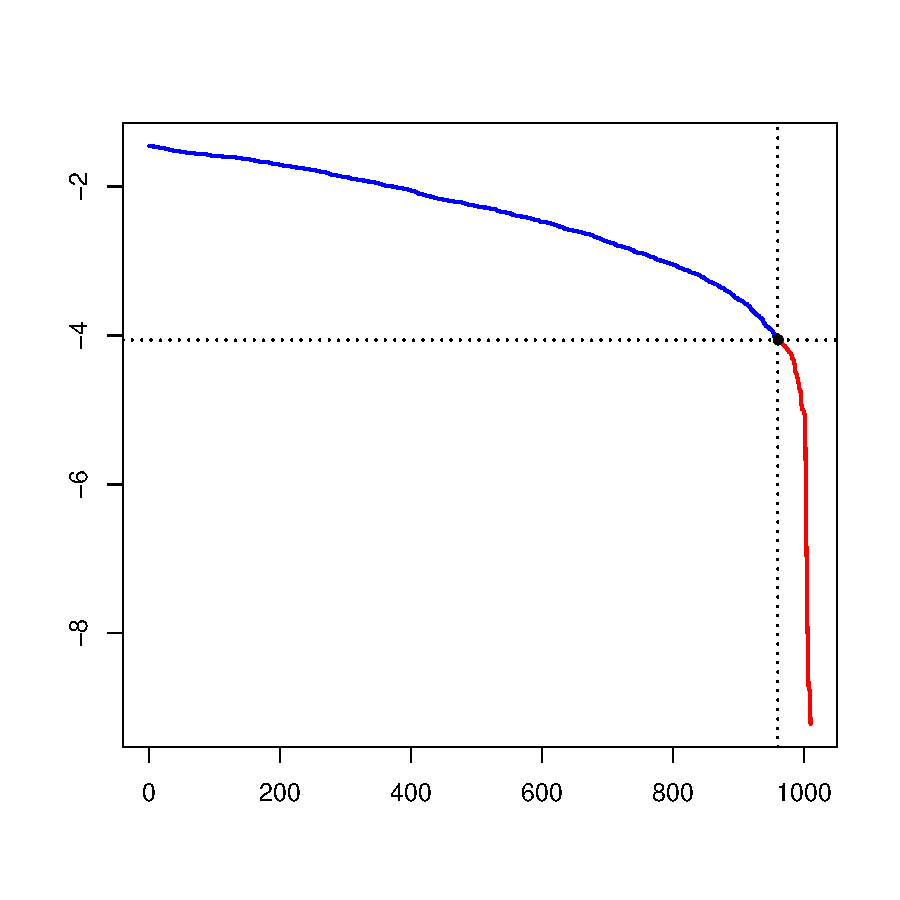
\includegraphics[width=12cm]{gmm-outliers-1}\hspace*{-2cm}
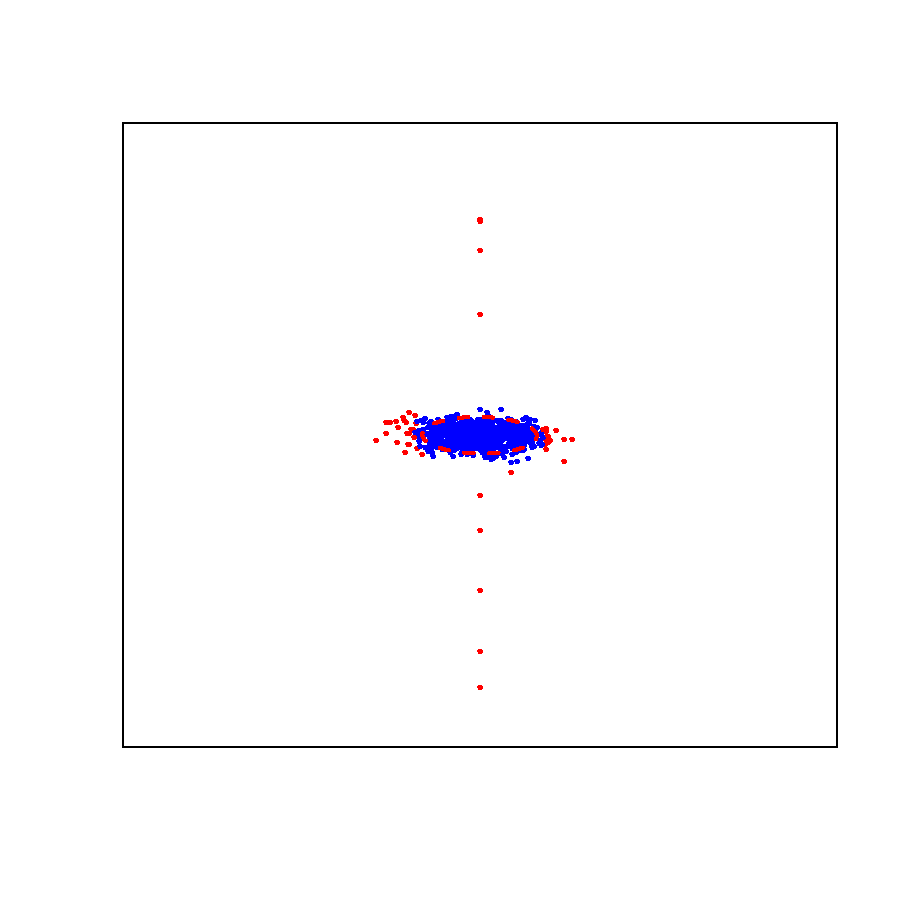
\includegraphics[width=12cm]{gmm-outliers-2}
\end{center}
\vspace*{-2cm}
Left pane shows ordered log likelihood of points and corresponding cut-off point. The right pane shows how the outlier elimination alter parameters. 


\foilhead[-2cm]{Choice of labels can be ambiguous}

\begin{center}
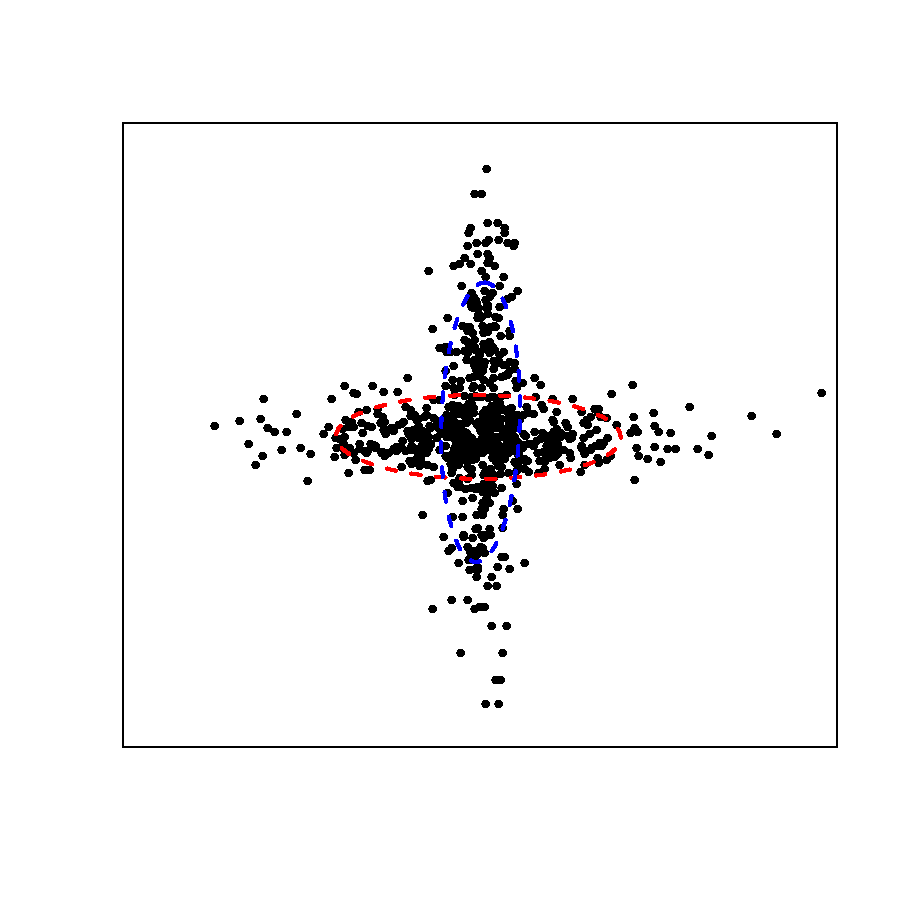
\includegraphics[width=12cm]{ambiguous-hc-1}\hspace*{-2cm}
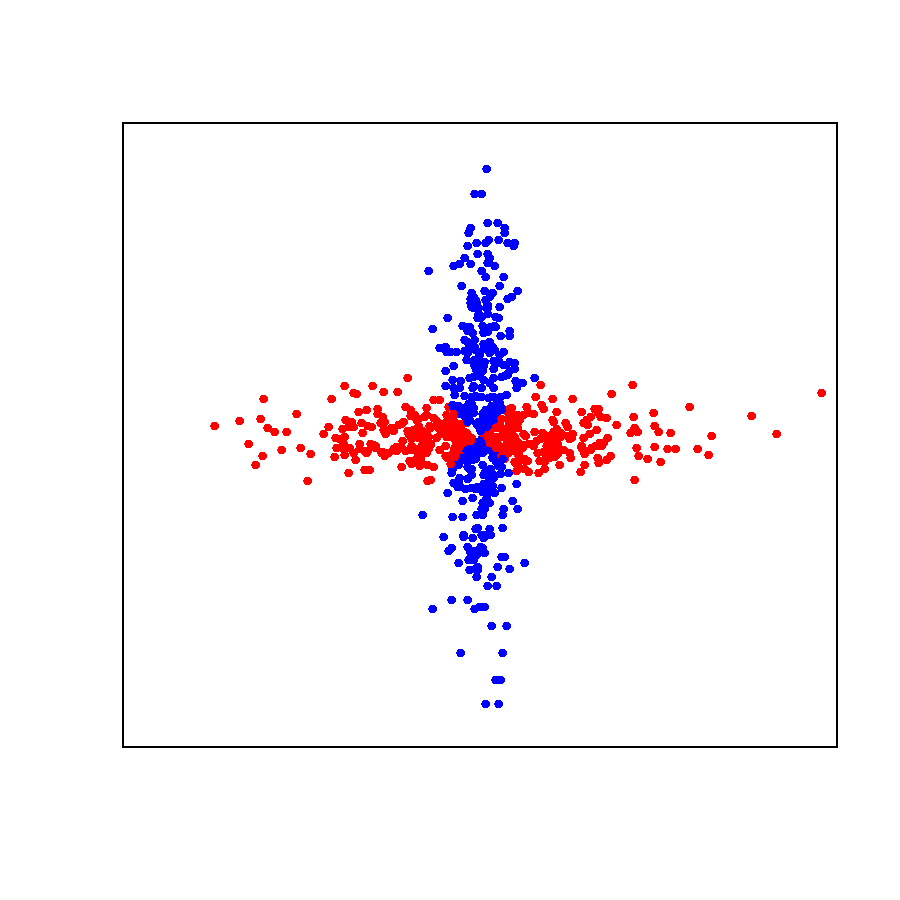
\includegraphics[width=12cm]{ambiguous-hc-2}
\end{center}
\vspace*{-2cm}

Sometimes the likelihoods for different sources are almost equal
\begin{triangles}
\item Label assignment is almost arbitrary 
\item Data points that belong to the cluster are not counted
\end{triangles}

\foilhead[-1cm]{Fractional weights as an alternative}

Data points should have different weighs based on the plausibility 
\begin{triangles}
\item Potential outliers should have low weights to limit their impact
\item Ambiguous points should impact the parameters of both clusters 
\item We should not prefer some data points to others in the algorithm
\end{triangles} 
\vspace*{2cm}

\textbf{First try.}
The most obvious choice for the weights are likelihoods
\begin{align*}
w_{ij}=\pd{\vec{x}_i|z_i=j,\vec{\Theta}_j}
\end{align*} 
but some data points have very low likelihoods for all clusters
\begin{triangles}
\item These data points would be largely ignored by the algorithm 
\end{triangles} 

\foilhead[-1cm]{The weighting scheme hides data}

\begin{center}
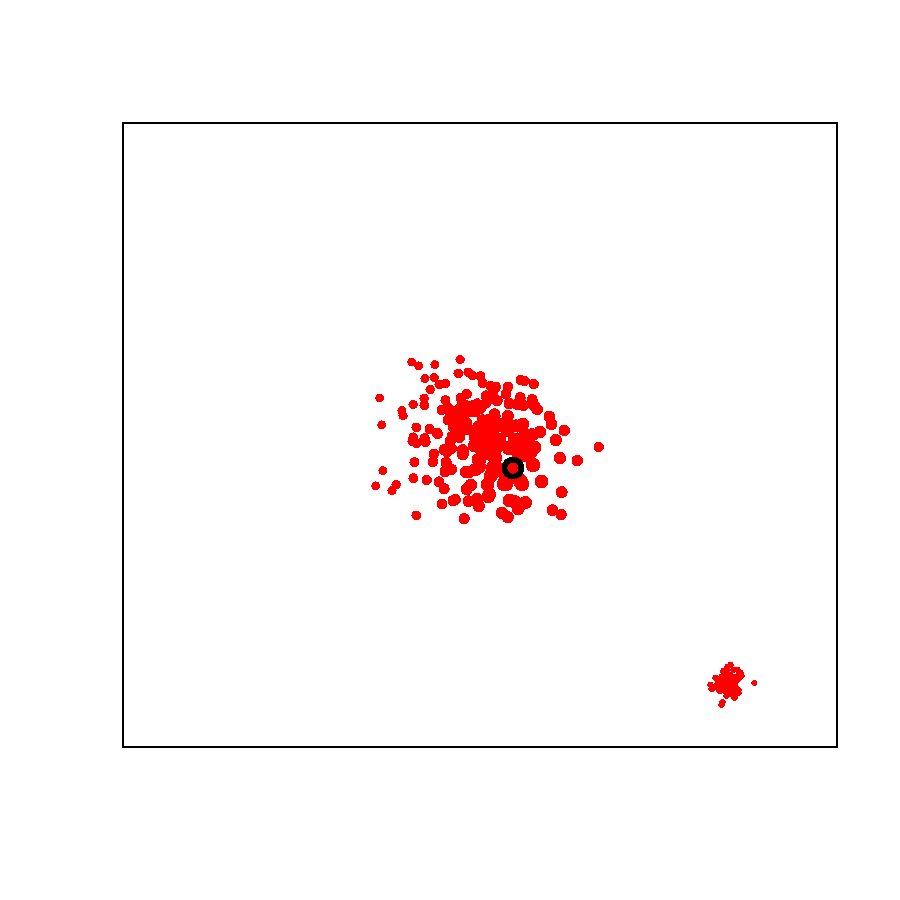
\includegraphics[width=12cm]{weighting-scheme-i-1}\hspace*{-2cm}
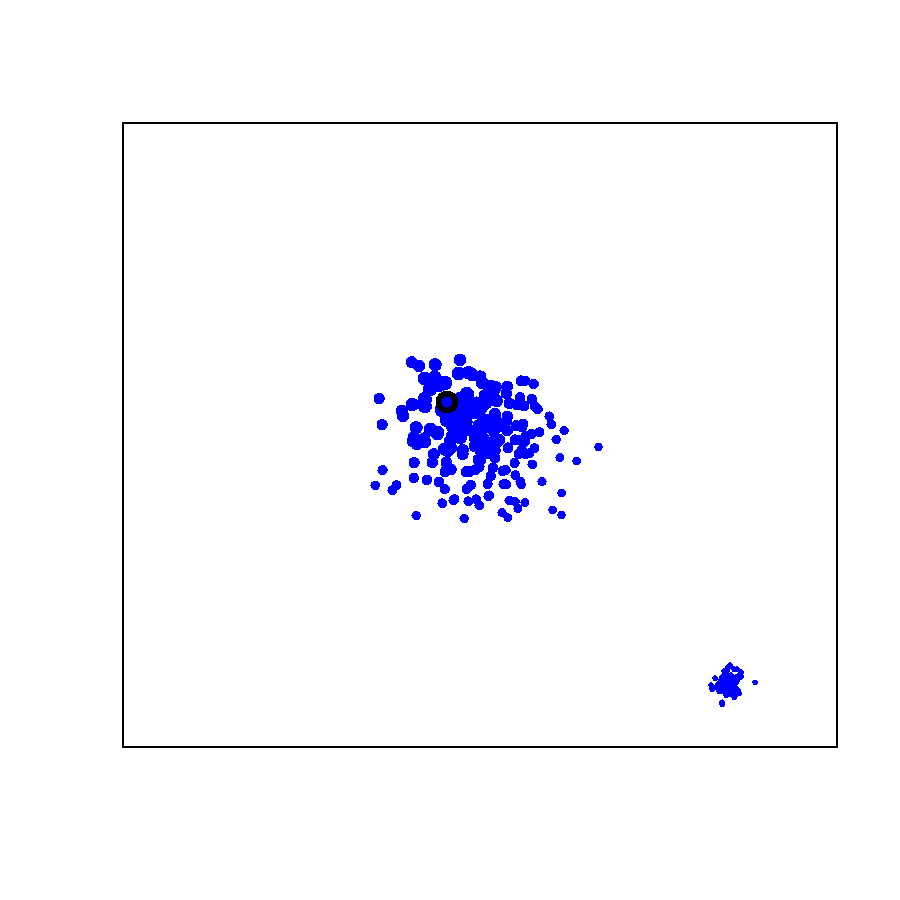
\includegraphics[width=12cm]{weighting-scheme-i-2}
\end{center}
\vspace*{-2cm}

The overall contribution of cluster points in south-east direction is small for both clusters and thus the cluster is never found by the the algorithm.




\foilhead[-1cm]{Fractional weights as an alternative}

Data points should have different weighs based on the plausibility 
\begin{triangles}
\item Potential outliers should have low weights to limit their impact
\item Ambiguous points should impact the parameters of both clusters 
\item We should not prefer some data points to others in the algorithm
\end{triangles} 
\vspace*{1cm}

\textbf{Second try.}
We can normalise the weights so that the sum up to one
\begin{align*}
w_{ij}=\frac{\pd{\vec{x}_i|z_i=j,\vec{\Theta}_j}}{\pd{\vec{x}_i|z_i=1,\vec{\Theta}_1}+\cdots+\pd{\vec{x}_i|z_i=k,\vec{\Theta}_k}}
\end{align*}

This weighting does not work if getting data points from some cluster is much more probable than from the other clusters.
\vspace*{-1cm} 



\foilhead[-1cm]{The weighting scheme ignores frequency}

\begin{center}
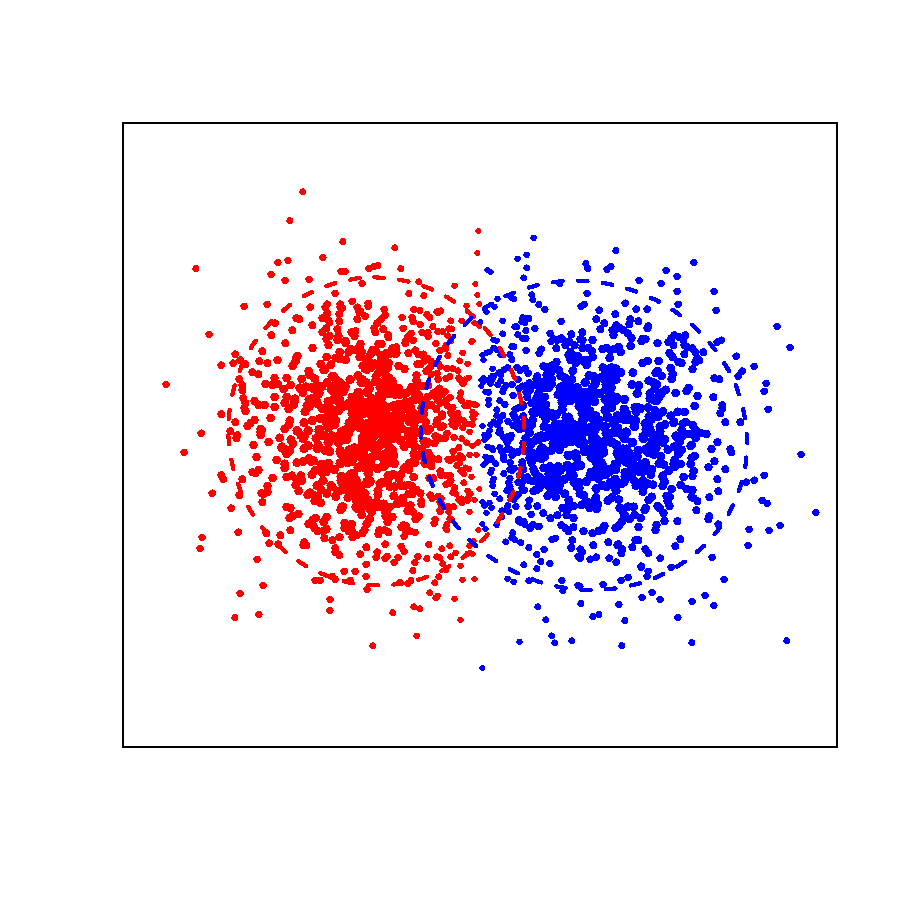
\includegraphics[width=12cm]{weighting-scheme-ii-1}\hspace*{-2cm}
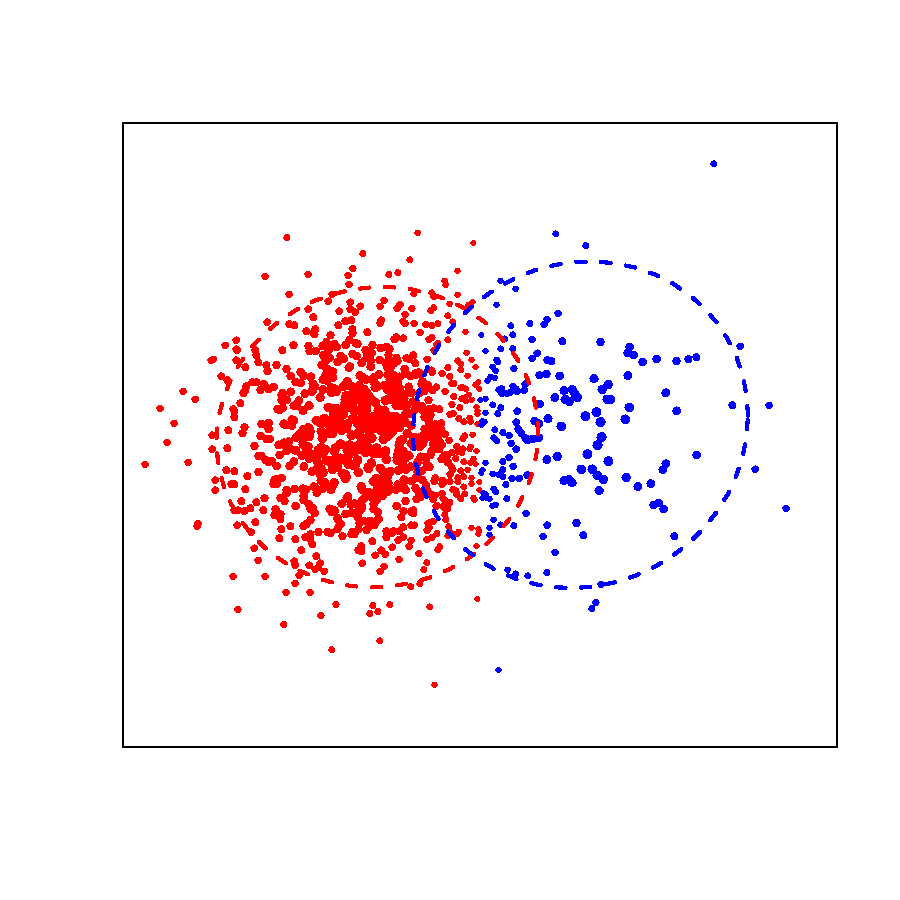
\includegraphics[width=12cm]{weighting-scheme-ii-2}
\end{center}
\vspace*{-2cm}

If the elements from one data source are rare then the elements form the ambiguous area are more likely to originate from the abundant source.
\vspace*{-1cm}  


\foilhead[-1cm]{Fractional weights as an alternative}

Data points should have different weighs based on the plausibility 
\begin{triangles}
\item Potential outliers should have low weights to limit their impact
\item Ambiguous points should impact the parameters of both clusters 
\item We should not prefer some data points to others in the algorithm
\end{triangles} 
\vspace*{1cm}

\textbf{Standard solution.}
We must take mixture proportions into account
\begin{align*}
w_{ij}&=\frac{\lambda_j\cdot\pd{\vec{x}_i|z_i=j,\vec{\Theta}_j}}{\lambda_1\cdot\pd{\vec{x}_i|z_i=1,\vec{\Theta}_1}+\cdots+\lambda_k\cdot\pd{\vec{x}_i|z_i=k,\vec{\Theta}_k}}\\
  &=\frac{\pd{\vec{x}_i,z_i=j|\vec{\Theta}}}{\pd{\vec{x}_i|\vec{\Theta}}}
  =\pd{z_i=j|\vec{x}_i,\vec{\Theta}}
\end{align*}
and thus the weight $w_{ij}$ is equal to label probability given $\vec{x}_i$ and $\vec{\Theta}$.\vspace*{-0.5cm}

\middlefoil{How to handle fractional\vspace{1.0ex}\\  weights?}

\foilhead[-1cm]{Naive implementation of fractional weights}

Under the independence assumption hard-clustering minimises 
\begin{align*}
F(\vec{z},\vec{\Theta}) =- \sum_{i=1}^n \log\pd{\vec{x}_i|z_i,\vec{\Theta}_{z_i}}
\end{align*}
To implement weights with precision $\frac{1}{\ell}$ we duplicate each data point $\ell$ times and modify label assignment step \textbf{M1}. The step \textbf{M2} remains same.  
\vspace*{1cm}

\textbf{E1 step} 
\begin{triangles}
\item Find weights for each $w_{ij}=\pr{z_i=j|\vec{x}_i,\vec{\Theta}}$
\item Compute integer counts $c_{ij}=\round{w_{ij}\cdot \ell}$ so that they add up to $\ell$.
\item For each data point $\vec{x}_i$ assign $c_{ij}$ copies to the cluster $j$.   
\end{triangles}

\foilhead[-1cm]{Implementation without data duplication}

\textbf{E1 step.} Compute fractional weights $w_{ij}=\pd{z_i=j|\vec{x}_i,\vec{\Theta}}$ and assign proportional number of point instances $\hat{w}_{ij}$ to each cluster.  

\textbf{M2 step.} Find parameters $\vec{\Theta}$ that minimise 
\begin{align*}
F_*(\vec{w},\vec{\Theta}) =-\sum_{i=1}^n\sum_{j=1}^k w_{ij} \log\pd{\vec{x}_i|z_i=j,\vec{\Theta}}
\end{align*}


\textbf{Convergence}
\begin{triangles}
\item M2 step clearly reduces the objective function.
\item It is \redsout{not} evident that E1 step does not increase the objective function. 
\item We need another way to establish covergence. 
\end{triangles}

\foilhead[-1cm]{Update steps for Gaussian mixture model}
\enlargethispage{1cm}

\textbf{E1 step.} Compute fractional weights $w_{ij}=\pd{z_i=j|\vec{x}_i,\vec{\Theta}}$ for each point
\begin{align*}
w_{ij}&=\frac{\lambda_j\cdot\pd{\vec{x}_i|z_i=j,\vec{\Theta}_j}}{\lambda_1\cdot\pd{\vec{x}_i|z_i=1,\vec{\Theta}_1}+\cdots+\lambda_k\cdot\pd{\vec{x}_i|z_i=k,\vec{\Theta}_k}}
\end{align*}
\vspace*{0.5cm}  



\textbf{M2 step.} Find parameters $\vec{\Theta}$ that minimise $F_*(\vec{w},\vec{\Theta})$ for fixed $\vec{w}$ where $\vec{w}$ denotes fractional multiplicity of labels:
\begin{align*}
&\begin{aligned}
n_j&=\sum_{i=1}^n w_{ij}\\
\lambda_j&= \frac{n_j}{n_1+\cdots+n_k}
\end{aligned}
&&\begin{aligned}
\vec{\mu_{j}}&=\frac{1}{n_j}\cdot\sum_{i=1}^n w_{ij}\vec{x}_{i}\\
\Sigma_{j}&=\frac{1}{n_j}\cdot X^t \mathsf{diag}(\vec{w}_{*j})X\\
\end{aligned}
\end{align*}
\vspace*{-0.5cm}  

\middlefoil{Why does this algorithm\vspace*{1ex}\\ work?}

\foilhead[-1cm]{Hard-clustering is non-optimal in theory}

\enlargethispage{1cm}
Assume that we can compute all likelihoods $\pd{\vec{x}_1,\vec{x}_2|\vec{z},\MMM_1}$ for two models

\begin{center}
\begin{tabular}{cccc}
Model    & $z_1$ & $z_2$ & $\mathrm{p}$\\
\hline
$\MMM_1$ & 0 & 0 & 0.18\\
$\MMM_1$ & 0 & 1 & 0.17\\
$\MMM_1$ & 1 & 0 & 0.14\\
$\MMM_1$ & 1 & 1 & 0.15\\
\hline
&&& \textbf{0.64}
\end{tabular}\hspace*{2cm}
\begin{tabular}{cccc}
Model    & $z_1$ & $z_2$ & $\mathrm{p}$\\
\hline
$\MMM_2$ & 0 & 0 & \textbf{0.24}\\
$\MMM_2$ & 0 & 1 & 0.04\\
$\MMM_2$ & 1 & 0 & 0.04\\
$\MMM_2$ & 1 & 1 & 0.04\\
\hline
&&& 0.36
\end{tabular}
\end{center}
Then the hard clustering algorithm chooses the model $\MMM_2$ although the overall plausibility of $\MMM_1$ is much higher if we are neutral. 

\textbf{Fix.} We should choose the model with the highest posterior probability
\begin{align*}
\pd{\vec{\Theta}|\vec{x}_1,\ldots,\vec{x}_n}=\sum_{\vec{z}}\pd{\vec{\Theta},\vec{z}|\vec{x}_1,\ldots,\vec{x}_n}
\end{align*}

\foilhead[-1cm]{Further analysis}

Now note that 
\begin{align*}
\pd{\vec{\Theta},\vec{z}|\vec{x}_1,\ldots,\vec{x}_n}=\frac{\pd{\vec{x}_1,\ldots,\vec{x}_n,\vec{z}|\vec{\Theta}} \cdot\pd{\vec{\Theta}}}{\pd{\vec{x}_1,\ldots,\vec{x}_n}}
\end{align*}
and thus if we do \emph{not have preferences over models} we get 
\begin{align*}
\pd{\vec{\Theta},\vec{z}|\vec{x}_1,\ldots,\vec{x}_n}=c(\vec{x}_1,\ldots,\vec{x}_n)\cdot\pd{\vec{x}_1,\ldots,\vec{x}_n,\vec{z}|\vec{\Theta}} 
\end{align*}
Hence, we can solve the optimisation task
\begin{align*}
P(\vec{\Theta})=\sum_{\vec{z}}\pd{\vec{x}_1,\ldots,\vec{x}_n,\vec{z}|\vec{\Theta}}\to\max 
\end{align*}

\foilhead[-1cm]{Decomposition into individual draws}
The maximisation task is hard, since $P(\vec{\Theta})$ has no nice form 
\begin{align*}
P(\vec{\Theta})&=\sum_{\vec{z}}\prod_{i=1}^n\pr{z_i|\vec{\Theta}}\cdot
\pd{\vec{x}_i|z_i,\vec{\Theta}_{z_i}}\\
&=\prod_{i=1}^n\sum_{j=1}^k\pr{z_i=j|\vec{\Theta}}\cdot
\pd{\vec{x}_i|z_i=j,\vec{\Theta}_{j}}
\end{align*}
Even the logarithm trick does not help
\begin{align*}
\log P(\vec{\Theta})&=
\sum_{i=1}^n\log\left(\sum_{j=1}^k\pr{z_i=j|\vec{\Theta}}\cdot
\pd{\vec{x}_i|\vec{z}_i=j,\vec{\Theta}_{j}}\right)
\end{align*}

\foilhead[-1cm]{Heuristic minimisation}

Lets assign an arbitrary probability distribution over labels $q(\vec{z})$ then we can formally provide a lower bound to the log-likelihood
\begin{align*}
\log \pd{\vec{\Theta}|\vec{x}_1,\ldots\vec{x}_n}%
&=\log\left(\sum_{\vec{z}}q(\vec{z})\cdot\frac{\pd{\vec{\Theta}, \vec{z}|\vec{x}_1,\ldots,\vec{x}_n}}{q(\vec{z})}\right)\\
&\geq \sum_{\vec{z}}q(\vec{z})\cdot\log\left(\frac{\pd{\vec{\Theta},\vec{z}|\vec{x}_1,\ldots,\vec{x}_n}}{q(\vec{z})}\right)=F(\vec{q},\vec{\Theta})
\end{align*}
Now if we manage to find $q(\vec{z})$ and $\vec{\Theta}$ that maximise $F(\vec{q},\vec{\Theta})$ we have located the set of model parameters where the sought log-likelihood $P(\vec{\Theta})$ must be quite high.


\foilhead[-1cm]{Further analysis}
The new minimisation target further decomposes into two separate parts
\begin{align*}
F(\vec{q},\vec{\Theta})= -\sum_{\vec{z}}q(\vec{z})\cdot\log q(\vec{z})+
 \sum_{\vec{z}}q(\vec{z})\cdot\log\left(\pd{\vec{z},\vec{\Theta}|\vec{x}_1,\ldots,\vec{x}_n}\right)
\end{align*}
and we can use two-step minimisation algorithm
\vspace*{1cm}

\textbf{E step.} Fix $\vec{\Theta}$ and find optimal weights $q(\vec{z})$ for all labels

\textbf{M step.} Fix all weights $q(\vec{z})$ and find parameters $\vec{\Theta}$ maximising $F(\vec{q},\vec{\Theta})$


\foilhead[-1cm]{What are optimal weights?}

It is well known fact that the term 
\begin{align*}
 \sum_{\vec{z}}q(\vec{z})\cdot\log\left(\frac{\pd{\vec{z},\vec{\Theta}|\vec{x}_1,\ldots,\vec{x}_n}}{q(\vec{z})}\right)
\end{align*}
is maximised only if 
\begin{align*}
q(\vec{z})&= c_*\cdot \pd{\vec{z},\vec{\Theta}|\vec{x}_1,\ldots,\vec{x}_n}=\pd{\vec{z}|\vec{\Theta},\vec{x}_1,\ldots,\vec{x}_n}
\end{align*}
Since the probabilities of labels decompose into the product so does $q(\vec{z})$
\begin{align*}
q(\vec{z})=\prod_{i=1}^n \pd{z_i|\vec{\Theta}_{z_i},\vec{x}_i}=\prod_{i=1}^n w_{iz_i}
\end{align*}
where the weights are the same as were in our \emph{practical algorithm}. 

\foilhead[-1cm]{What are optimal parameters?}

For fixed weights $q(\vec{z})$ the first term in $F(\vec{q},\vec{\Theta})$ is constant and thus optimal set of parameters can be found by maximising
\begin{align*}
 \sum_{\vec{z}}q(\vec{z})\cdot\log\left(\pd{\vec{z},\vec{\Theta}|\vec{x}_1,\ldots,\vec{x}_n}\right)
\end{align*}
The latter is equivalent to the following maximisation task
\begin{align*}
 \sum_{\vec{z}}q(\vec{z})\cdot\log\left(\pd{\vec{x}_1,\ldots,\vec{x}_n, \vec{z}|\vec{\Theta}}\right)
\end{align*}
which can be further decomposed into a simpler sum
\begin{align*}
\sum_{i=1}^n \sum_{\vec{z}\in\ZZZ} q(\vec{z})\cdot\log\left(\pd{\vec{x}_i,z_i|\vec{\Theta}}\right)
&=\sum_{i=1}^n \sum_{\vec{z}\in\ZZZ}\prod_{\ell=1}^n w_{\ell z_\ell}\cdot\log\left(\pd{\vec{x}_i,z_i|\vec{\Theta}}\right)
\enspace.
\end{align*}


\foilhead[-1cm]{Lower-bound regularly coincides with probability}

Observe the second factor in the sum after E-step to get further insight  
\begin{align*}
F(\vec{q},\vec{\Theta})&= \sum_{\vec{z}}q(\vec{z})\cdot\log\left(\frac{\pd{\vec{\Theta},\vec{z}|\vec{x}_1,\ldots,\vec{x}_n}}{q(\vec{z})}\right)\\
&=\sum_{\vec{z}}q(\vec{z})\cdot\log\left(\frac{\pd{\vec{\Theta},\vec{z}|\vec{x}_1,\ldots,\vec{x}_n}}{\pd{\vec{z}|\vec{\Theta},\vec{x}_1,\ldots,\vec{x}_n}}\right)\\
&= \sum_{\vec{z}}q(\vec{z})\cdot\log\left(\frac{\pd{\vec{\Theta},\vec{z}|\vec{x}_1,\ldots,\vec{x}_n}}{\pd{\vec{z}|\vec{\Theta},\vec{x}_1,\ldots,\vec{x}_n}}\right)\\
&= \sum_{\vec{z}}q(\vec{z})\cdot\log\left(\pd{\vec{\Theta}|\vec{x}_1,\ldots,\vec{x}_n}\right)\\
&= \colorbox{orange}{$\log\left(\pd{\vec{\Theta}|\vec{x}_1,\ldots,\vec{x}_n}\right)$}
\end{align*}


\foilhead[-1cm]{Connection with the hard-clustering algorithm}

The hard-clustering algorithm assigns zero-one probabilities to different labelings $\vec{z}$ which can be formalised as products of zero-one weights $w_{ij}$. Thus the parameters are still chosen by maximising
\begin{align*}
\sum_{i=1}^n \sum_{\vec{z}\in\ZZZ}\prod_{\ell=1}^n w_{\ell z_\ell}\cdot\log\left(\pd{\vec{x}_i,z_i|\vec{\Theta}}\right)
\enspace.
\end{align*}
Soft-clustering (EM-algorithm) is just a more general maximisation task.

Maximisation task can be converted back to hard-clustering problem by rounding fractional weights to integers.
\begin{triangles}
\item This leads to the dataset with repeated data samples. 
\item We can still use the update steps for hard clustering.
\end{triangles}

\end{document}

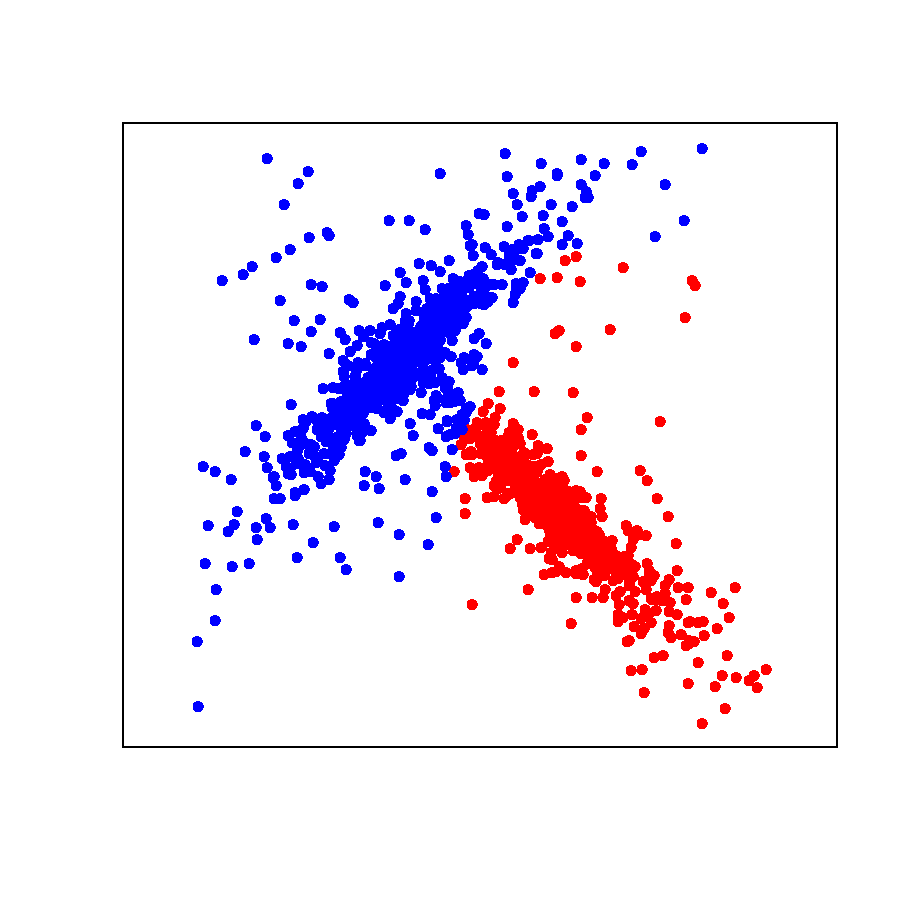
\includegraphics[width=7.5cm]{hard-gmm-4}
corrupted-gmm-1.pdf

\illustration[scale=0.9, trim = 5cm 2.5cm 5cm 2cm, clip]{shooting-target}

Find the true target for each shooter given that errors in all directions are equiprobable and distributed according to normal distribution.\vspace*{-1cm}

\foilhead[-0cm]{Target reconstruction in shooting}

\illustration[scale=0.9, trim = 5cm 2.5cm 5cm 2cm, clip]{shooting-target-precise}

Reconstruction of the true targets is straightforward when we know the origin of individual shots. We discuss later how to do it exactly.\vspace*{-1cm}

\foilhead[-0cm]{Target reconstruction in shooting}

\illustration[scale=0.9, trim = 5cm 2.5cm 5cm 2cm, clip]{shooting-target-blinded}

Reconstruction of the true targets is much harder if we have to guess the origin of shots by ourselves. This task is known as clustering.\vspace*{-1cm}


\foilhead[-1cm]{Naive probabilistic model}

\begin{triangles}
\item There are $k$ different data sources $\DDD_1,\ldots,\DDD_k$
\item Each data source has a fixed centre $\vec{\mu}_j\in\RR^d$
\item For each data point noise $\varepsilon_t\gets\NNN(0,\sigma)$ for each coordinate
\item To sample data from the distribution $\DDD_j$, we output $\vec{x}=\vec{\mu}_j+\vec{\varepsilon}$ 
\end{triangles}
\vspace*{1cm}

\textbf{Correponding mathematical model.} Let $z_1,\ldots, z_n$ denote assigned labels and $\vec{x}_1,\ldots,\vec{x}_n$ locations of individual data points. Then
\begin{align*}
\pd{\vec{x}_i|z_i=j,\vec{\mu}_j,\sigma}&=\prod_{t=1}^d\frac{1}{\sqrt{2\pi}\sigma}\cdot\exp{-\frac{(x_{it}-\mu_{jt})^2}{-2\sigma^2}}\\
\pd{\vec{x}_1,\ldots,\vec{x}_n|\vec{z},\vec{\mu}_1,\ldots,\vec{\mu}_1,\sigma}&=\prod_{i=1}^n
\prod_{t=1}^d\frac{1}{\sqrt{2\pi}\sigma}\cdot\exp{-\frac{(x_{it}-\mu_{z_it})^2}{-2\sigma^2}}
\end{align*}


\foilhead[-1cm]{Corresponding minimisation task}
\enlargethispage{1cm}
Again it makes sense to maximise log-likelihood instead of likelihood
\begin{align*}
\log \pd{\vec{x}_1,\ldots,\vec{x}_n|\vec{z},\vec{\mu}_1,\ldots,\vec{\mu}_1,\sigma}&= C(\sigma) - 
\sum_{i=1}^n
\sum_{t=1}^d\frac{(x_{it}-\mu_{z_it})^2}{2\sigma^2}
\end{align*}
The latter is equivalent to the following minimisation task:
\begin{align*}
\sum_{i=1}^n\norm{\vec{x}_i-\vec{\mu}_{z_i}}^2\to\min
\end{align*}
where  the labelling $\vec{z}_1,\ldots,\vec{z}_n$ and cluster centres $\vec{\mu}_1,\ldots,\vec{\mu}_k$ is sought.

\textbf{Minor problem:} The optimisation task is known to be NP-hard.


\foilhead[-1cm]{Two-step gradient decent algorithm}

\textbf{Observation.} If the labels are fixed then it is easy to find optimal placement of cluster centres. First, note that we can separately optimise the location of each centre, as the sum decomposes into independent minimisation targets:  
\begin{align*}
\sum_{i=1}^n\norm{\vec{x}_i-\vec{\mu}_{z_i}}^2=\sum_{i\in\III_1}\norm{\vec{x}_i-\vec{\mu}_{1}}^2+\cdots+\sum_{i\in\III_k}\norm{\vec{x}_i-\vec{\mu}_{k}}^2
\end{align*}
For each individual minimisation target $F_j$ we can compute the derivatives
\begin{align*}
\frac{\partial F_j}{\partial \mu_{js}}=\sum_{i\in\III_j}\sum_{t=1}^d\frac{\partial}{\partial \mu_{js}}(x_{it}-\mu_{jt})^2=
-\sum_{i\in\III_j}2(x_{is}-\mu_{is})
\end{align*}
and thus $\vec{\mu}_j$ is the mean of all data points in the cluster  


\foilhead[-1cm]{Two-step gradient decent algorithm}

\textbf{Observation.} If cluster centres are fixed then it straightforward to find best label for each data point. We must choose the closest cluster centre $\vec{\mu}_j$.
\vspace*{2cm}


\textbf{K-means clustering algorithm}
\begin{triangles}
\item[1.] Choose a good initial positions for cluster centres
\item[2.] For each data point $\vec{x}_i$ find the closest cluster centre $\vec{\mu}_j$ and set $z_i=j$
\item[3.] Recompute cluster centres as averages over data points belonging to it
\item[4.] Repeat from the step 2 until nothing changes.
\item[5.] Repeat with different starting points and report the best result   
\end{triangles}

\foilhead[-2.0cm]{The algorithm really works}

\centerline{
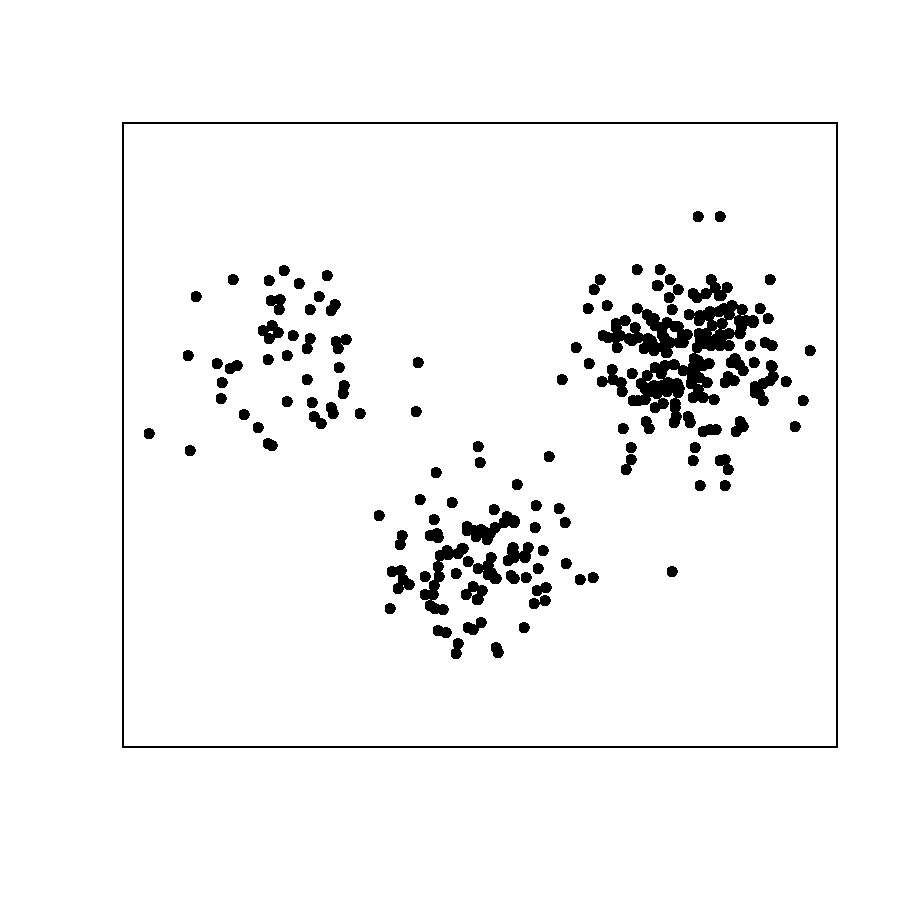
\includegraphics[scale=0.6]{kmeans-1}\hspace*{-1.7cm}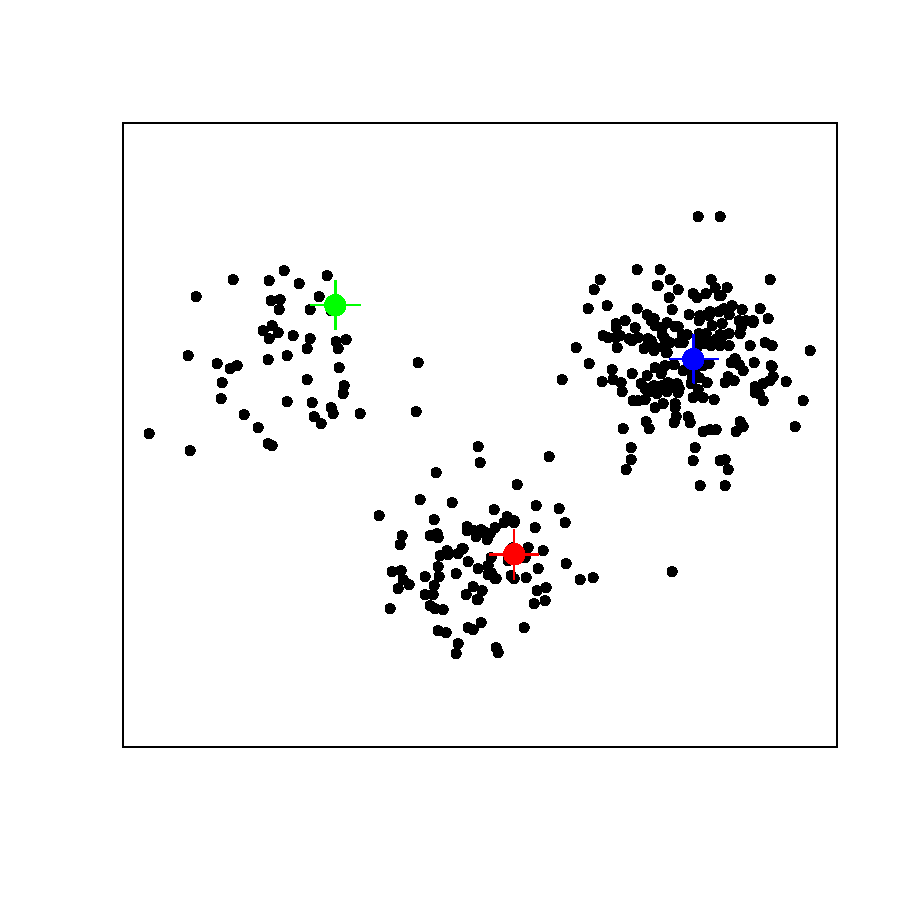
\includegraphics[scale=0.6]{kmeans-2}
\vspace*{-2.6cm}}

\centerline{
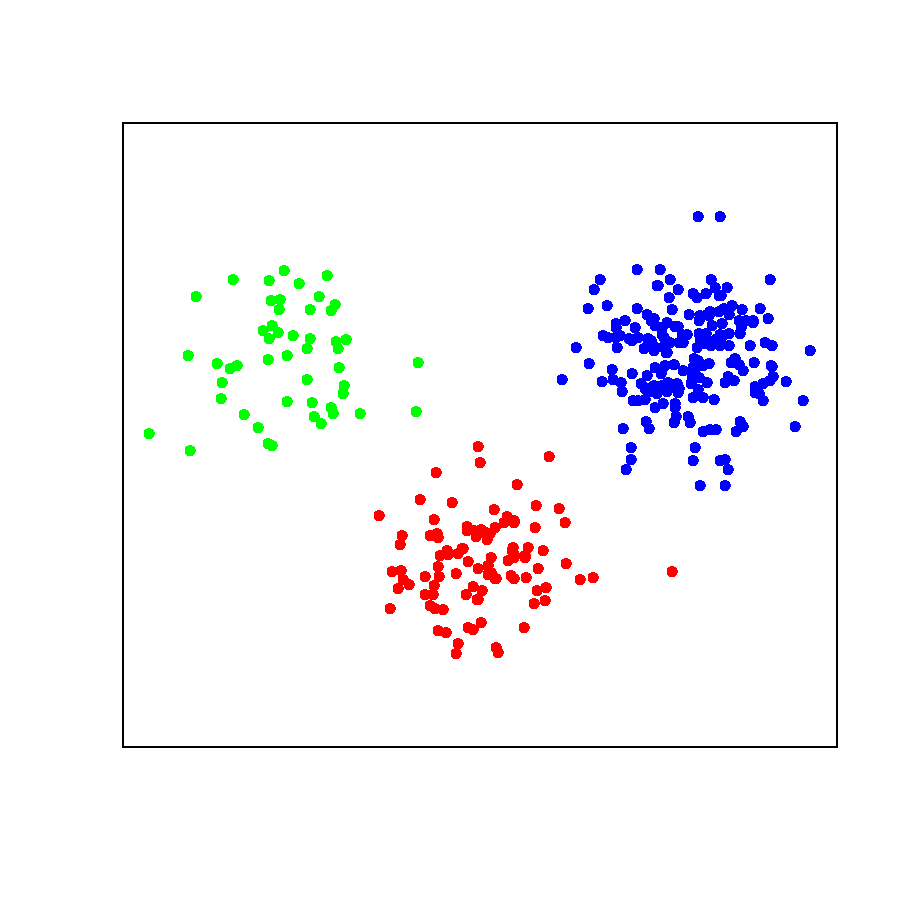
\includegraphics[scale=0.6]{kmeans-3}\hspace*{-1.7cm}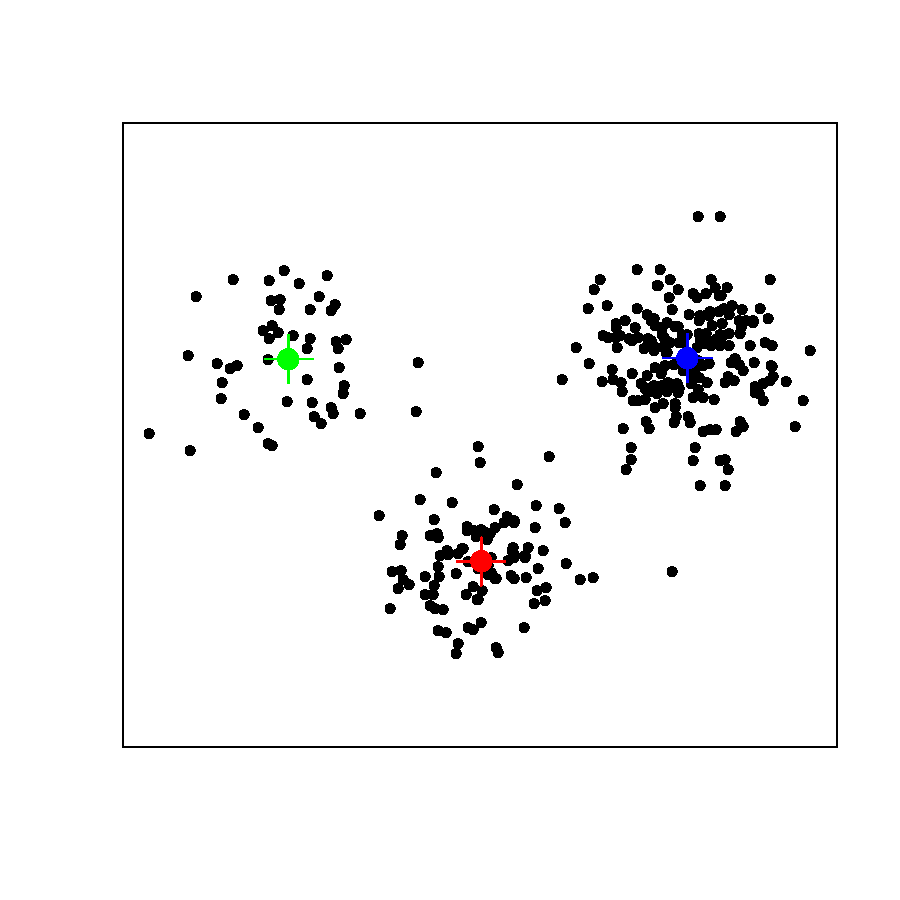
\includegraphics[scale=0.6]{kmeans-4}
\vspace*{-3.2cm}}

\foilhead[-1cm]{Example of suboptimal behaviour}

\centerline{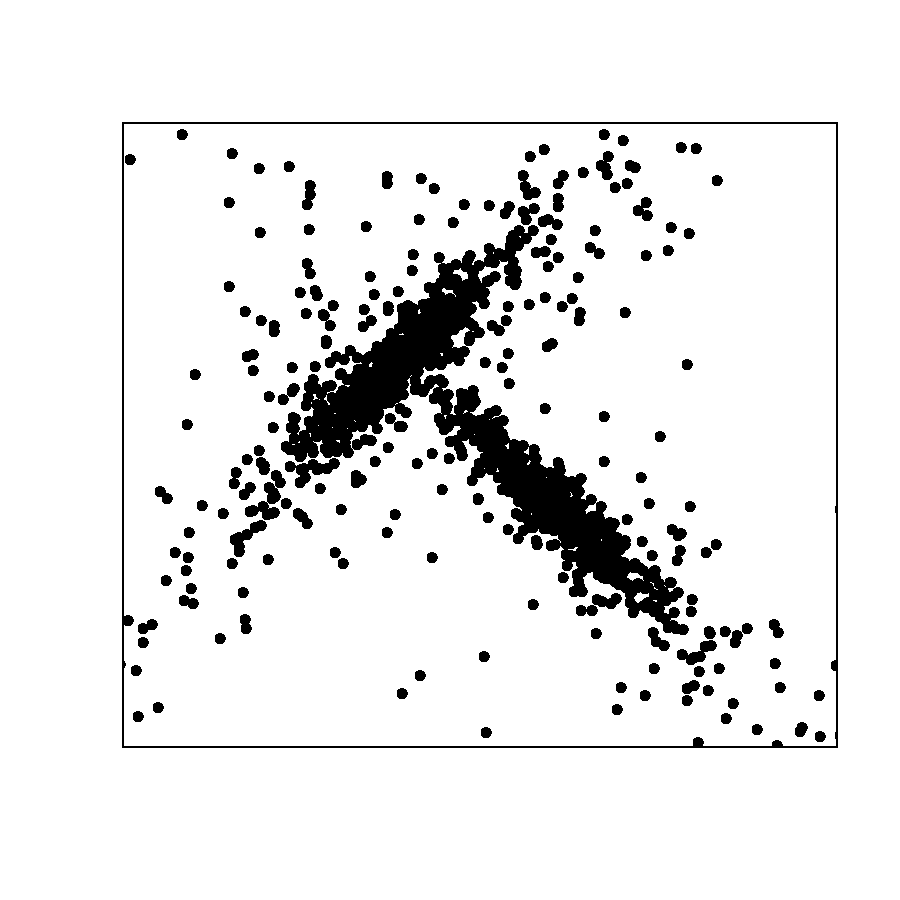
\includegraphics[scale=0.8]{kmeans-failure-1}\hspace*{-1.7cm}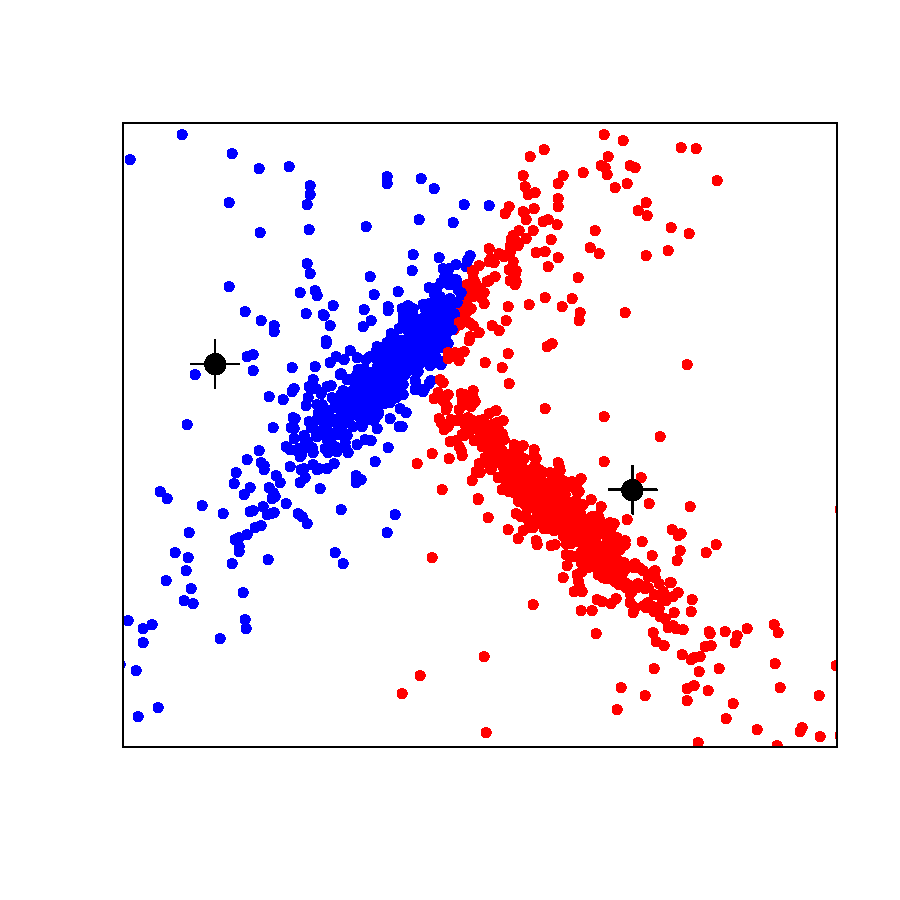
\includegraphics[scale=0.8]{kmeans-failure-2}}
\vspace*{-2cm}

K-means algorithm fails if clusters are elongated or one clusters have different density. In both cases the assumptions are not satisfied. 


\foilhead[-1cm]{Model for elongated clusters}

\begin{triangles}
\item Components of the underlying true noise  are samples as $\varepsilon_i\gets\NNN(0,1)$
\item Noise is reshaped using linear transformation $\vec{\varepsilon}_*=A\vec{\varepsilon}$
\item The final output is generated as $\vec{x}=\vec{\mu}+\vec{\varepsilon}_*$ 
\end{triangles}
\vspace*{1cm}


\textbf{Correponding mathematical model.} It is straightforward to express the corresponding probability density function
\begin{align*}
\pd{\vec{x}|\vec{\mu},A}&=\frac{1}{(\det A^TA)^{1/2}}\cdot\prod_{t=1}^d\frac{1}{\sqrt{2\pi}}\cdot\exp{-\frac{\varepsilon_t^2}{2}}\\
\pd{\vec{x}|\vec{\mu},A}&=\frac{1}{(2\pi)^{d/2}(\det AA^T)^{1/2}}\cdot\exp{-\frac{1}{2}\cdot (\vec{x}-\vec{\mu})A^{-T}A^{-1}(\vec{x}-\vec{\mu})}
\end{align*} 
where $\Sigma=AA^T$ is known as correlation matrix


\foilhead[-1cm]{Maximum likelihood estimates}

Multivariate normal distribution (\emph{coloured Gaussian noise}) $\NNN(\vec{\mu}, \Sigma)$ is completely determines by the centre $\vec{\mu}$ and correlation matrix $\Sigma$. 

It is straightforward though tedious to verify that parameter values that maximise the likelihood of data $\vec{x}_1,\ldots,\vec{x}_n$ can be competed as follows
\begin{align*}
\vec{\mu}&=\frac{1}{n}\cdot\sum_{i=1}^n \vec{x}_i\\
\Sigma&=\frac{1}{n}\cdot X^T X
\end{align*}
where $X$ is a $n\times d$ data matrix obtained by staking $\vec{x}_1^T,\ldots,\vec{x}_n^T$.

\foilhead[-1cm]{Gaussian mixture model}

\begin{triangles}
\item There are $k$ different data sources $\DDD_1,\ldots,\DDD_k$
\item Each data source has a fixed centre $\vec{\mu}_j\in\RR^d$ and covariance matrix $\Sigma_j$
\item To sample data from  $\DDD_j$, we output $\vec{x}=\vec{\mu}_j+\vec{\varepsilon}$ for $\varepsilon\gets\NNN(\vec{0},\Sigma_j)$ 
\item A data point is sampled form the distribution $\DDD_j$ with probability $\lambda_j$
\end{triangles}

\vspace*{1cm}


\textbf{Correponding hard-clustering task.} Find model parameters $\vec{\Theta}$ and labels $\vec{z}$ such that the likelihood of the data is maximal:
\begin{align*}
\pr{\vec{x}_1,\ldots,\vec{x}_n|\vec{z},\vec{\Theta}}\to \max
\end{align*}


\foilhead[-1cm]{Two-step gradient decent algorithm}

\textbf{Observations} 
\begin{triangles}
\item If parameters $\vec{\Theta}$ are fixed it straightforward to find best label for each data point. We must choose $z_i$ such that $\pd{\vec{x}_i|\vec{\mu}_i,\Sigma_i}\to \max$.
\item If labels are fixed then we can individually adjust the parameters $\vec{\mu}_j$ and $\Sigma_j$ for clusters. Mixture fractions can be recomputed as $\lambda_j=\abs{\III_j}/n$.
\end{triangles}

\vspace*{0.5cm}


\textbf{Corresponding hard-clustering algorithm}
\begin{triangles}
\item[1.] Choose a good initial values for cluster parameters
\item[2.] For each data point $\vec{x}_i$ find the best cluster $j$ and set $z_i=j$
\item[3.] Recompute cluster parameters over data points belonging to it
\item[4.] Update cluster weights $\lambda_1,\ldots,\lambda_k$ 
\item[5.] Repeat from the step 2 until nothing changes
\item[6.] Repeat with different starting points and report the best result   
\end{triangles}
\vspace*{-0.5cm}


\foilhead[-2.0cm]{The algorithm really works}

\centerline{
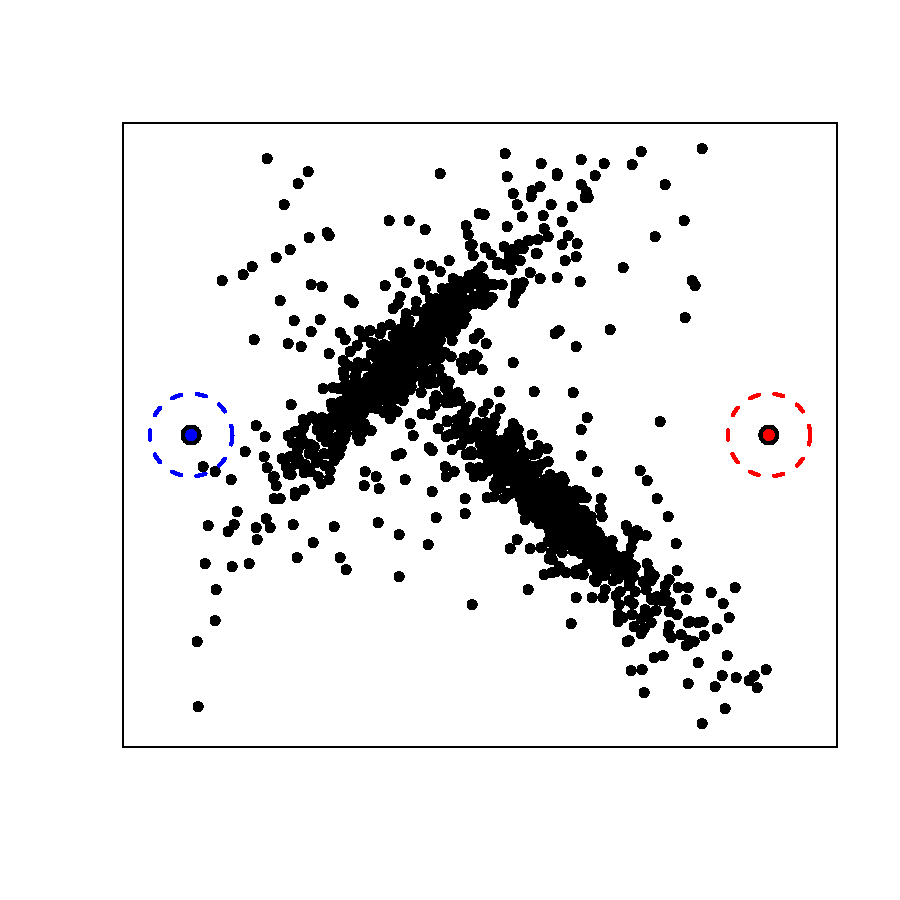
\includegraphics[scale=0.6]{hard-gmm-1}\hspace*{-1.7cm}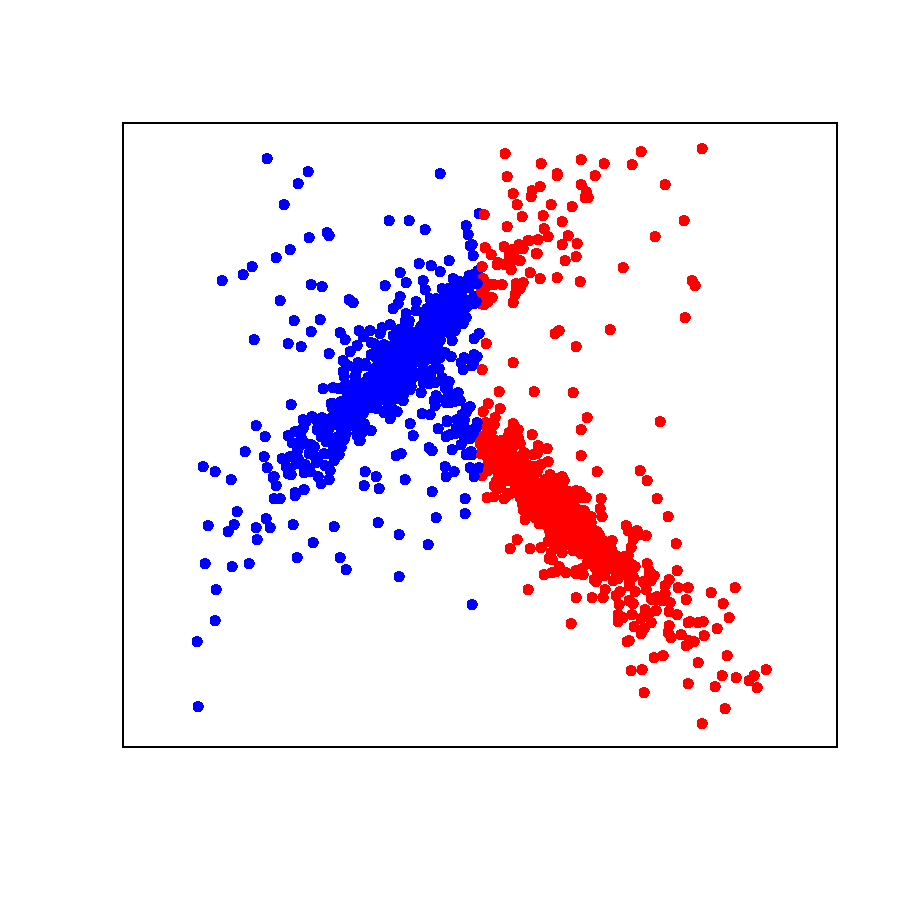
\includegraphics[scale=0.6]{hard-gmm-2}
\vspace*{-2.6cm}}

\centerline{
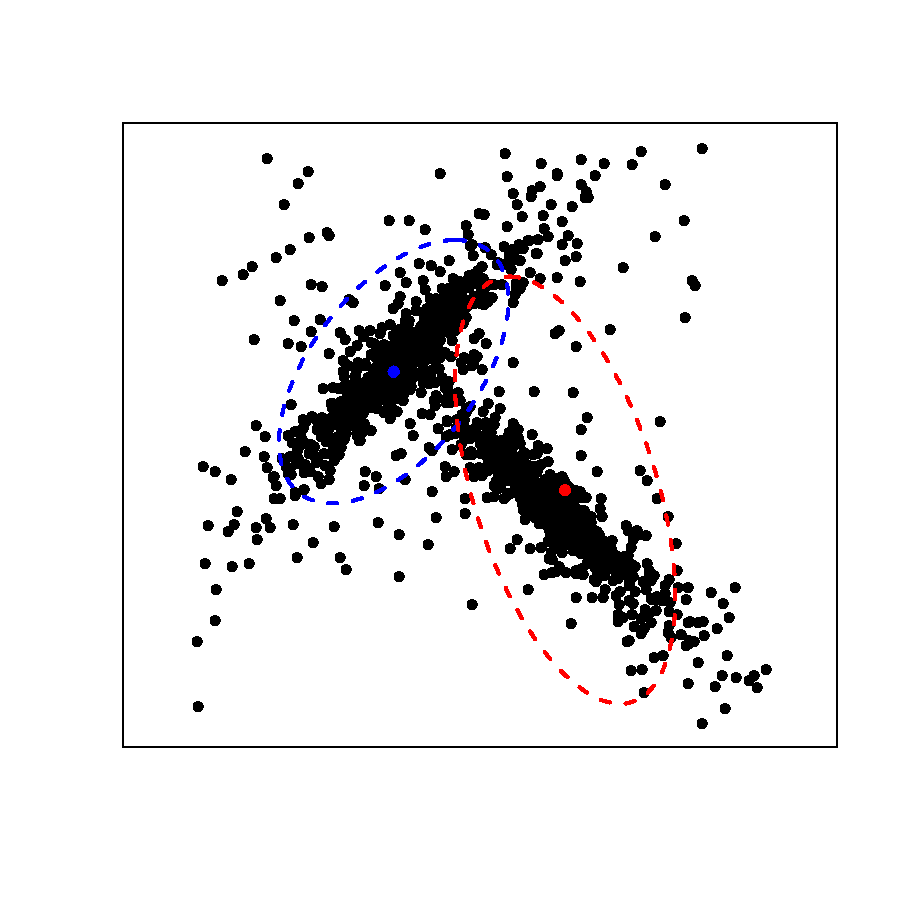
\includegraphics[scale=0.6]{hard-gmm-3}\hspace*{-1.7cm}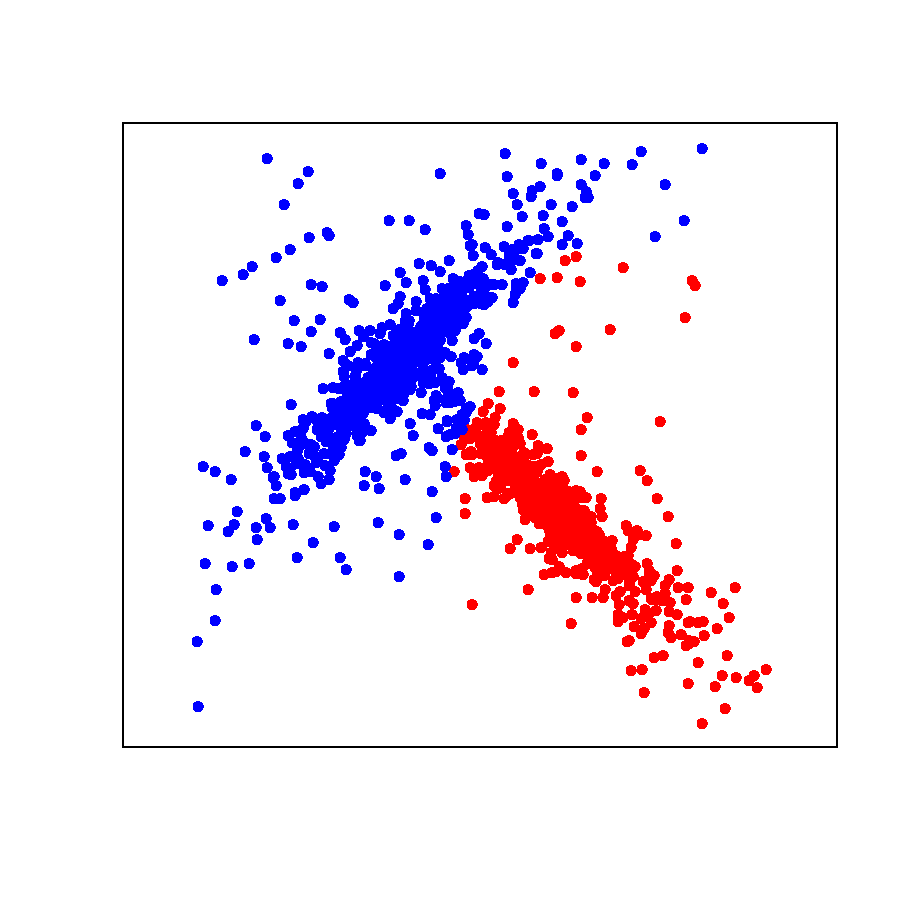
\includegraphics[scale=0.6]{hard-gmm-4}
\vspace*{-3.2cm}}

\foilhead[-1cm]{Hard datasets for the algorithm}

\centerline{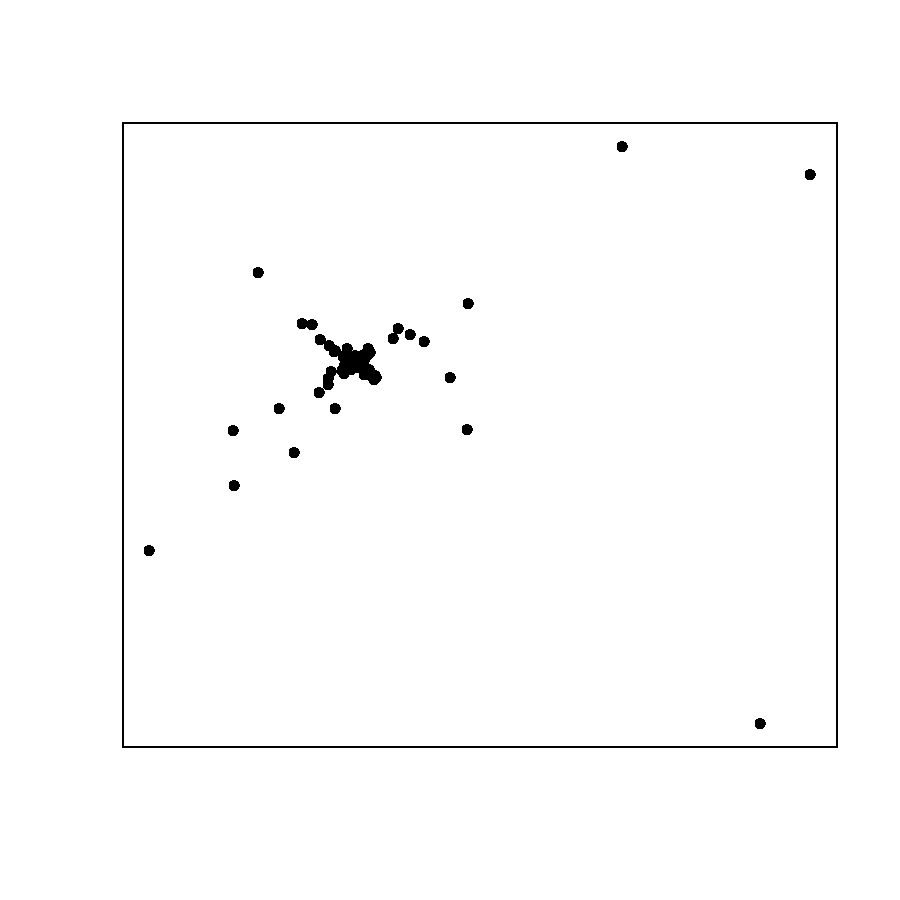
\includegraphics[scale=0.8]{hard-gmm-failure-1}\hspace*{-1.7cm}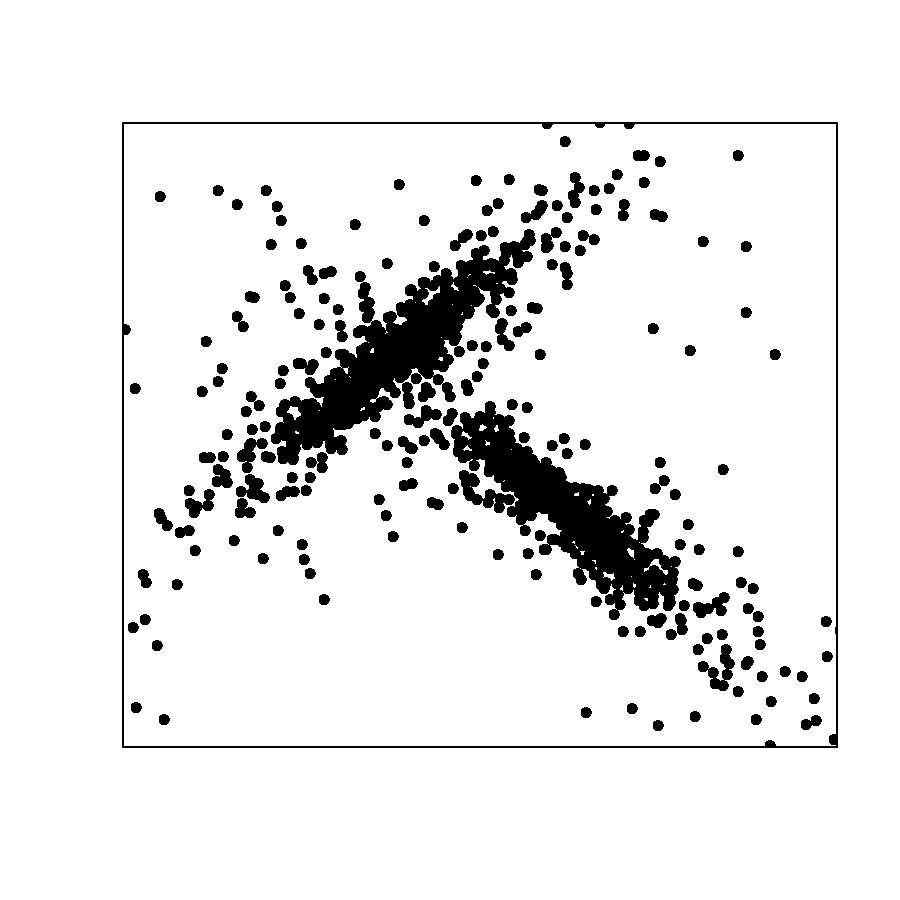
\includegraphics[scale=0.8]{hard-gmm-failure-2}}
\vspace*{-1cm}

Few extreme values can completely offset the hard-clustering algorithm. The latter is the weakness of the Gaussian mixture model.\vspace*{-0.5cm}


\end{document}
